% !TeX root = ../main.tex

\chapter{緒論}

地球作為一顆動態的行星,其內部動力學相當複雜。地球動力學(Geodynamics)由地球(Geo-)與動力(dynamics)兩個詞所組成,顧名思義為探討地球內部的動力過程,以及地球內部物質受力後所發生的變形作用。
查理斯萊爾爵士(Sir Charles Lyell)在《地質學原理(Principles of Geology)》(\citealp{lyell1837principles})一書中提到「現在是通往過去的一把鑰匙」,表示過去所發生的地質事件與現在進行中的地質作用皆相同。

人類在很早之前便知道地球有動態過程,例如地震與火山爆發。
早期的地球科學研究侷限於地表觀察,儘管在牛頓力學成為自然科學的顯學後,以物理基礎定量描述自然現象與作用力已被廣泛應用,但由於地質作用之時間尺度遠超乎當時定年技術的範疇,故地球內部之構造活動尚無人知曉。
至19世紀,隨著人類在實驗與測量技術上的突破,藉由物理方法探測地球內部的技術才開始被應用到對地球內部的觀察,然而當時的地球物理學門與地質科學是完全分開的領域。
直到板塊構造學說被提出,地球內部的驅動力可以藉由隱沒板塊水平運動所實現,顛覆地質構造由垂直運動所主導的地槽學說概念。
至此,地球科學從定性的地質描述轉變成定量的物理展現,由板塊運動所引起的地質現象在時間與空間上有最大程度的整合,該理論被稱為地球科學上的科學革命。
從此,人類可以藉由簡單的物理力學模型描述已發生的地質事件,近一步預測未來的地質構造。

計算機模擬是在計算機上執行數學建模的過程,被用來預測物理系統與現實世界的行為與結果。
該技術可以在成本較少的狀態下實現結果的推斷,量化模型實現後的不確定性,因此,計算機模擬已經大量被運用在社會科學、醫療科學、工程學與自然科學。
地球動力學研究中,使用電腦建立地質模型,並且利用數值方法計算模擬地球內部的演化,便是一種計算機模擬。對於相對簡單的過程,模型中的物理方程式可以使用解析解或半解析解模型(e.g., \citealp{samuel2006oscillating}; \citealp{montesi2007mantle}),不過如果需要描述較複雜的物理機制,在既定物理假設下的數學方程組只能用數值方法進行計算(詳見第二章),此時模型稱作地球動力學的數值模擬(geodynamic processes with numerical techniques)(\citealp{101Geodynamics})。

自板塊構造學說被提出以來,實現動態地球的隱沒帶系統無論在巨觀尺度下構造的演化或微觀尺度下礦物的排列與物質置換皆是人類致力於研究的目標。
作為板塊構造運動的主要驅動力,隱沒帶系統是主要的火山與地震活動來源,過程牽扯到多尺度地質作用事件,包含緩慢的岩石脫水相變、岩漿演化與瞬態的岩石破裂。
隱沒帶數值模擬可以利用已知的物理約束與岩石流變行為預測隱沒帶內部的演化過程(\citealp{Gerya2011}),然而建立模型除了需要對地球內部的理論有一定成熟的基礎外,電腦運算的技術是另一個需要突破的重點。
自第一篇二維隱沒帶數值模型文章(\citealp{minear1970thermal})發布以來,隨著地球科學研究在實驗與資料品質上的日益上升,以及硬體技術大幅提升,地球動力學數值模型研究已經是發展成熟且被廣泛應用的地球科學學門。
因此,近年來隱沒帶數值模型會根據不同研究目標考慮隱沒系統中的複雜作用,例如岩漿作用、物質交換、岩石變質作用與板塊脫水作用等,在多領域理論上實現更大程度的概念整合。

\section{背景}\label{背景}

板塊構造學說主張地球最外層之剛性殼體---岩石圈為地表水平運動單位。
因地球內部的熱引起重力不穩定而導致岩石圈在軟流圈上水平運動(\citealp{jordan1978composition})。
岩石圈斷裂成許多剛性塊體,該塊體被稱為板塊。
大部分由板塊水平運動所引起的變形作用發生在板塊邊界。
在聚合板塊邊界,板塊發生破壞,包含碰撞與隱沒。
在分離板塊邊界,板塊發生增生,代表構造為中洋脊擴張現象。
錯動邊界中板塊不會顯著發生增生與破壞,代表構造為轉型斷層。

在聚合板塊邊界,溫度較冷的板塊隱沒進入地球內部,同時因溫度差所引起的密度差導致重力不穩定區形成,其中溫度越低,密度越大。
隱沒板塊上方的聚合板塊稱為上覆板塊(overriding plate, upper plate)。
隨著隱沒板塊帶著較冷物質進入地函深處,周圍壓力逐漸上升,岩石發生相變,隱沒板塊因成分與溫度與地函物質不同,溫度上的差異造成更大的重力不穩定。
在同等深度下,海洋地殼上的玄武岩(basalt)最終相變成榴輝岩(eclogite)相,其為變質岩中密度最大的岩石,約落在3600-3800 kg$\cdot$m$^{-3}$之間,比重遠大於周圍地函。
所有的隱沒帶P-T路徑皆會通過榴輝岩相區(\citealp{gerya2002exhumation}; \citealp{syracuse2010global}; \citealp{penniston2015global})(見圖\ref{fig::global_subduction_eclogite})。
玄武岩相變榴輝岩的克拉伯隆斜率(Clapeyron slope)大於零(見圖\ref{fig::global_subduction_eclogite}),該相變會在隱沒板塊上較低溫的區域發生,所以於隱沒帶剖面上的同等深度中,在相變影響與溫度影響的加持下,造成隱沒板塊有足夠大的重力不穩定成為隱沒板塊持續下沉進入地球內部更深處的驅動力。
隱沒板塊為板塊移動與張裂的主要驅動力(\citealp{turcotte2002geodynamics}),作為岩石圈上最巨大的不均質構造,隱沒帶將許多地表的物質帶入地球內部,在岩石圈與軟流圈之間發生複雜的物理與化學作用。
隱沒板塊上的沉積物隨著周遭環境壓力與溫度逐漸升高而發生壓密作用(compaction),同時隱沒板塊上的岩石因壓力增大而將孔隙水排出,釋放進入弧前地殼區域; 在更深處,隱沒板塊上的含水礦物發生脫水作用,這些流體被釋放進入地函中,部分流體導致蛇紋岩化橄欖岩(serpentinitzed peridotite)生成,另外部分流體降低地函橄欖岩熔點,致使上覆板塊側岩石發生部分熔融,生成岩漿上升至地表,形成火山島弧。
隱沒帶中所產生的各種作用皆會對隱沒板塊動力學造成影響,故自然界中上部地函以上之隱沒幾何剖面有相當大的相異性,有許多原因影響隱沒傾角與隱沒曲率(\citealp{schellart2020control})。

平坦隱沒(Flat slab subduction)是一種特殊的隱沒帶,有別於一般的隱沒板塊由於重力不穩定而下沉進入地函,平坦隱沒系統中的隱沒板塊在地函淺部(<200公里)出現一段趨近於水平的幾何構造,該水平段可長達400公里。
\citet{barazangi1976}利用南美洲區域震源位置資料判斷秘魯與智利下方的隱沒板塊處於水平狀態,是為最早發現平坦隱沒的研究。
以下將介紹平坦隱沒,並且定義本研究中的平坦隱沒。

\begin{figure*}[hp]
    \centering
    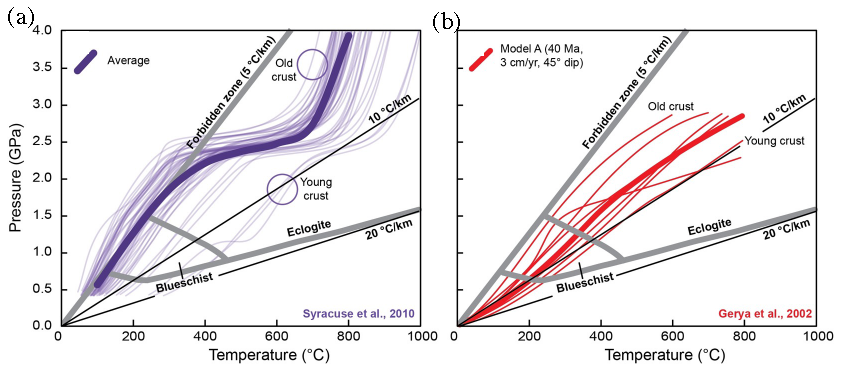
\includegraphics[width=6in]{global_subduction_eclogite.pdf}
    \caption[全球隱沒板塊頂部的預測P-T路徑圖,摘自\citet{penniston2015global}]{
    全球隱沒板塊頂部的預測P-T路徑圖,摘自\citet{penniston2015global}。圖中標示每公里5$^\circ$、10$^\circ$、20$^\circ$的地溫梯度與藍閃岩、榴輝岩溫壓位置。(a)來自\citet{syracuse2010global}的全球隱沒板塊P-T路徑圖(紫色線)。(b)來自\citet{gerya2002exhumation}的模型,紅色線代表不同年齡的隱沒板塊P-T路徑圖。
    }
    \label{fig::global_subduction_eclogite}
\end{figure*}

\section{平坦隱沒定義}\label{平坦隱沒定義}

地球內部的隱沒傾角在地域上變化極大。本研究對\textsl{slab 2.0} (\citealp{hayes2018slab2})全球模型中切出152條垂直於海溝的隱沒帶剖面(剖面位置參考自\citealp{Hu2020}),計算深度0-150 公里、距離海溝800公里內的隱沒帶傾角,以每5度為一間隔,獲得全球隱沒帶傾角分佈圖,如圖\ref{fig::number of tracsects}所示,全球只有大約$13\%$的隱沒帶傾角低於$20^\circ$。

目前學界並沒有明確的平坦隱沒定義,因此過去研究較少將低傾角隱沒帶與平坦隱沒分開討論,以往的數值模型多直接計算隱沒板塊在特定深度的斜率,一旦傾角低於特定值則視為平坦隱沒。
然而,隱沒板塊角度變化僅是最初步的隱沒帶特徵之一,隱沒帶中的幾何形狀更能展現隱沒帶的熱構造。
在上述的剖面中,將隱沒帶初步分成三類: 0-19$^\circ$、20-39$^\circ$、40-69$^\circ$,分別是為低傾角隱沒帶、正常隱沒帶與高傾角隱沒帶。
低傾角隱沒帶分別落在阿拉斯加、日本四國、卡斯卡迪亞(Cascadia)、墨西哥、新幾內亞以及安地斯隱沒帶上,\citet{schellart2020control}另外將低傾角隱沒帶分成兩種類型,在深度150 公里以上有兩個鉸鏈點(hinge)與三個鉸鏈點的隱沒板塊段,如圖\ref{fig::slab profile}所示。

\begin{figure*}[ht!]
    \centering
    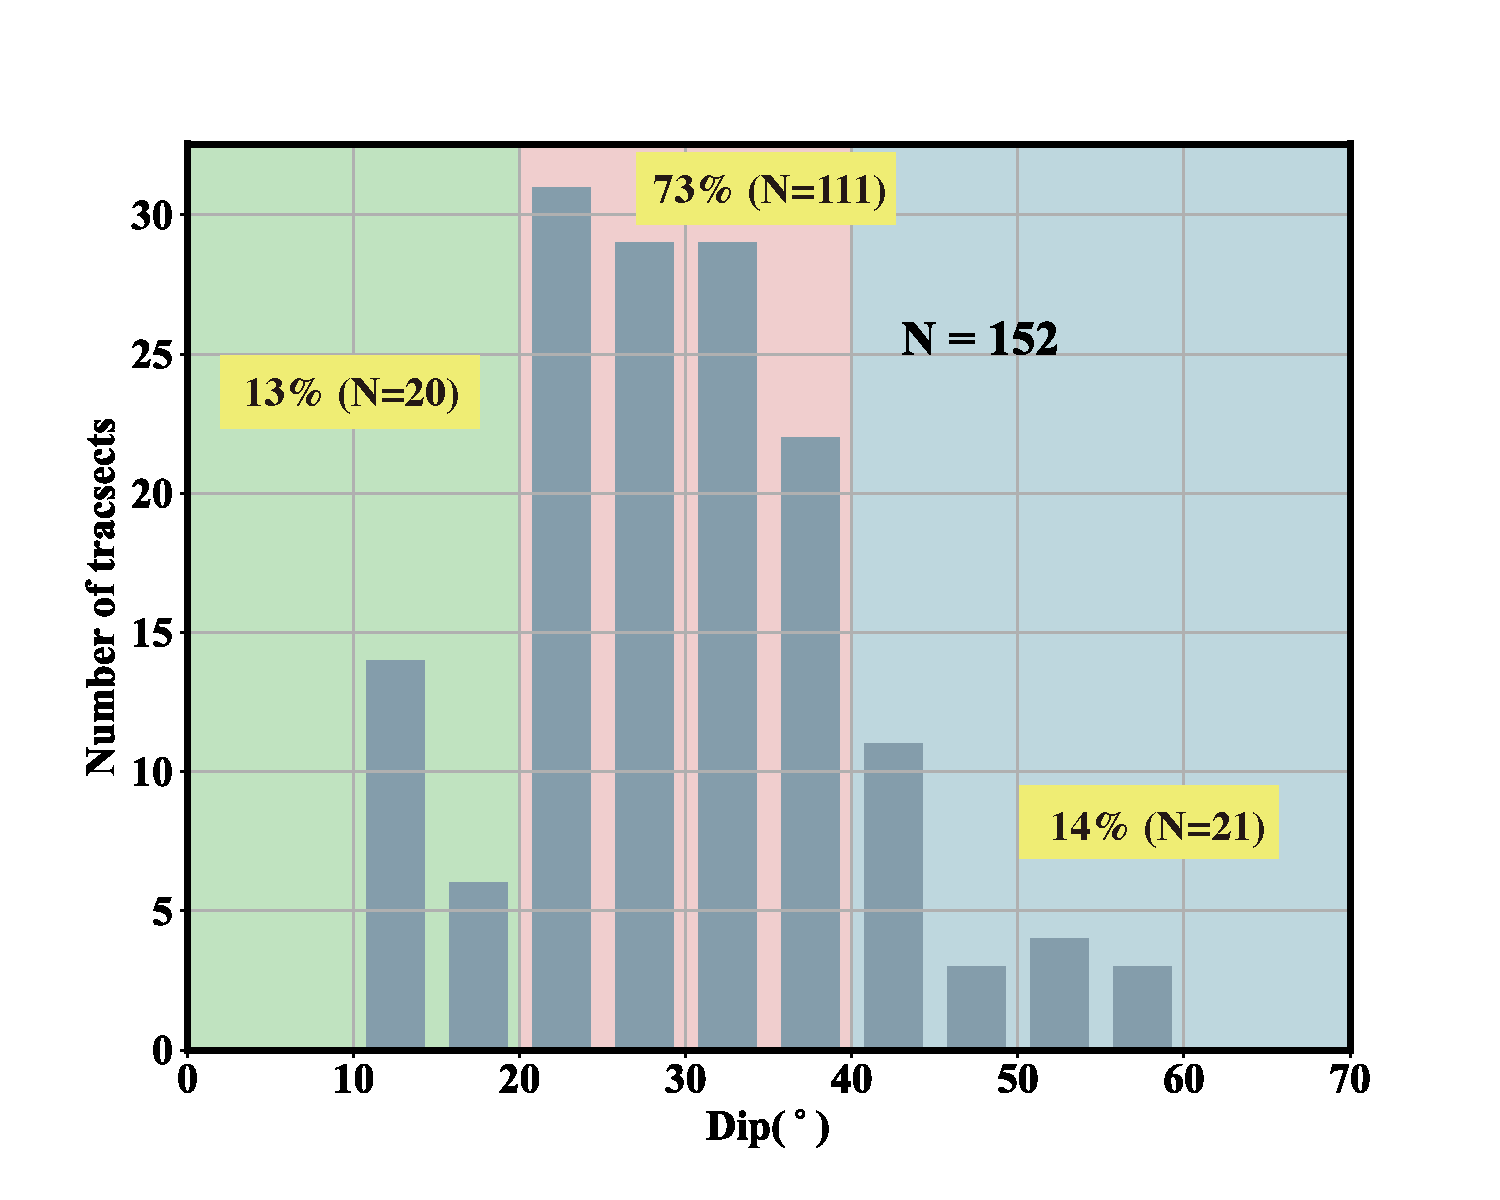
\includegraphics[width=4in]{chapter3_01.pdf}
    \caption[全球152條隱沒帶剖面傾角長條分布圖]{全球152條隱沒帶剖面傾角長條分布圖,其中綠底為隱沒剖面傾角低於20$^{\circ}$的剖面個數,佔整體13$\%$;粉紅底為剖面傾角介於20$^{\circ}$-39$^\circ$之間的剖面個數,佔整體$73\%$,粉藍底則為剖面傾角高於$40^\circ$的剖面個數,佔總體$14\%$。}
    \label{fig::number of tracsects}
\end{figure*}

\citet{schellart2020control}是少數將平坦隱沒與低傾角隱沒分開討論的研究,在他的定義中,相對於低傾角隱沒帶,大部分活躍的隱沒板塊具有一個鉸鏈點,接近海溝且下凹,如圖\ref{fig::slab profile}。
從圖\ref{fig::slab profile}可見,低傾角隱沒板塊會有兩個下凹鉸鏈點,第一個鉸鏈點接近海溝且呈現平緩不明顯的下凹,第二個鉸鏈點在距海溝幾百公里遠處,曲率明顯、板塊下凹進入深部地函,如圖\ref{fig::slab profile},阿拉斯加、卡斯卡迪亞、日本四國與新幾內亞等地區皆屬於此類。
另外在少數區域,隱沒板塊會有三個鉸鏈點,第一個鉸鏈點靠近海溝且下凹,第二個鉸鏈點深度較深且呈現上凹,被視為是平坦隱沒的開始端,在這兩個鉸鏈點中隱沒板塊傾角正常。
第三個鉸鏈點與第二個鉸鏈點深度相近,水平距離通常超過100公里以上,其曲率下凹的特徵代表著平坦隱沒的結束,平坦隱沒的距離與深度由第二與第三鉸鏈點所決定,如圖\ref{fig::slab profile}所示,智利、秘魯與墨西哥等地區屬於此類,在過去曾經被\citet{Manea2017}所討論。


\begin{figure*}[hbp]
    \centering
    \includegraphics[width=6in]{Slab_2.0_v1.pdf}
    \caption[slab 2.0 模型與四條參考剖面,改編自\citet{schellart2020control}]{slab 2.0 模型與四條參考剖面,改編自\citet{schellart2020control}。其中(a)為馬尼拉隱沒帶剖面,(b)為阿拉斯加隱沒帶剖面,(c)為加勒比板塊隱沒帶剖面,(d)為秘魯隱沒帶剖面。}
    \label{fig::slab profile}
\end{figure*}


然而由於過去研究對隱沒板塊鉸鏈點與曲率並沒有詳細定義,因此本研究並不採用上述的方式定義平坦隱沒,而是使用反曲點(Inflection point),方便後續對轉動力矩(見\ref{計算數值模型中的轉動力矩}節)進行比對,並且從數學面向來看更具有平坦(flat)的意義。
其中,反曲點的定義為連續曲線上穿越切線的點,亦即曲線二次微分等於0的點。
本研究將具有三個反曲點的隱沒段視為平坦隱沒,隱沒板塊曲線上除了具有兩個下凹特徵外,包含在兩側下凹隱沒中有一近乎平坦的隱沒段,有別於低傾角隱沒段的上下界深度落差可達50公里,其隱沒板塊在一固定深度幾乎維持水平狀態持續逾百公里以上。
為了確保數值模型中隱沒板塊是否符合平坦隱沒定義,本研究利用數學定義判斷平坦隱沒是否存在。
假設隱沒板塊為連續函數,令隱沒板塊方程式為$f(x)$, 其中$(x_{1},f(x_{1}))$, $(x_{2},f(x_{2}))$為x方向上最大的兩個反曲點(見圖\ref{fig::flat slab definition})。若為平坦隱沒,需同時滿足:

1. 最大兩個反曲點水平距離需大於100公里($\mid x_{1}-x_{2}\mid > 100 \ km$)。

2. 對整段隱沒板塊微分,其斜率的絕對值小於0.2之連續距離需大於50公里,該連續段稱為平坦隱沒之平坦段長度,其深度中位數稱為平坦段深度。

\begin{figure*}[ht!]
    \centering
    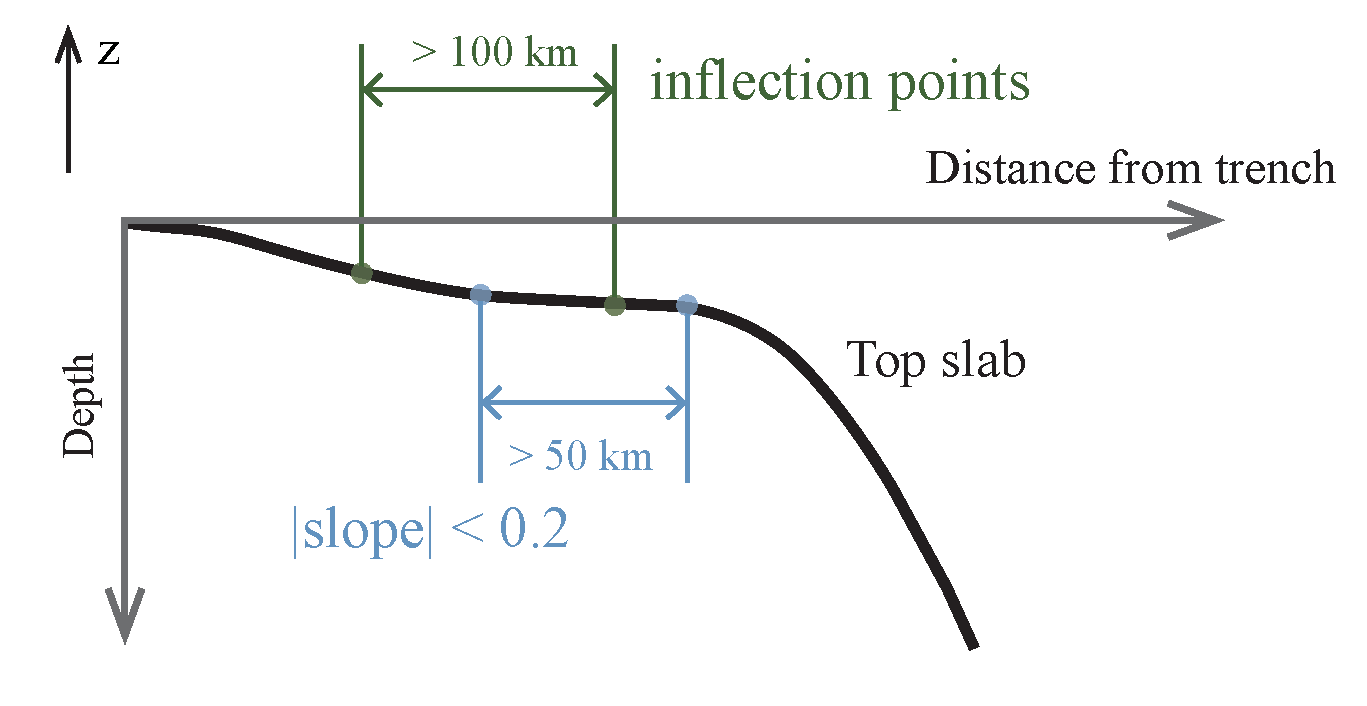
\includegraphics[width=6in]{flat_slab_definition.pdf}
    \caption[本研究中平坦隱沒的定義示意圖]{本研究中平坦隱沒的定義示意圖。綠色點表示隱沒板塊頂部上的反曲點,藍色點為隱沒板塊頂部上斜率絕對值小於0.2內最大連續範圍段的起點與終點。}
    \label{fig::flat slab definition}
\end{figure*}

如前所述,過往研究對平坦隱沒並沒有確切定義,絕大多數對平坦隱沒的判斷依據皆是以在固定深度範圍內隱沒板塊角度低於15-20度便視為平坦隱沒,然而這種定義除了無法分辨低傾角隱沒與平坦隱沒外,所選取的隱沒板塊深度範圍是另一種可變參數,結果較為發散。
重新定義平坦隱沒能夠用更具物理意義的方式觀察平坦隱沒在板塊運動中的各種動力影響。
藉由上述的定義方式,本研究重新分析152條隱沒剖面,結果表示只有科克斯板塊(Cocos plate)隱沒帶上的墨西哥區域與納茲卡板塊(Nazca plate)隱沒帶上的秘魯與智利區域有平坦隱沒的現象。

因此,接下來本研究以探討這三個區域的隱沒帶為主,其地理位置標示於圖\ref{fig::flat_slab_vol}的黃色框框中。

\begin{figure*}[hp]
    \centering
    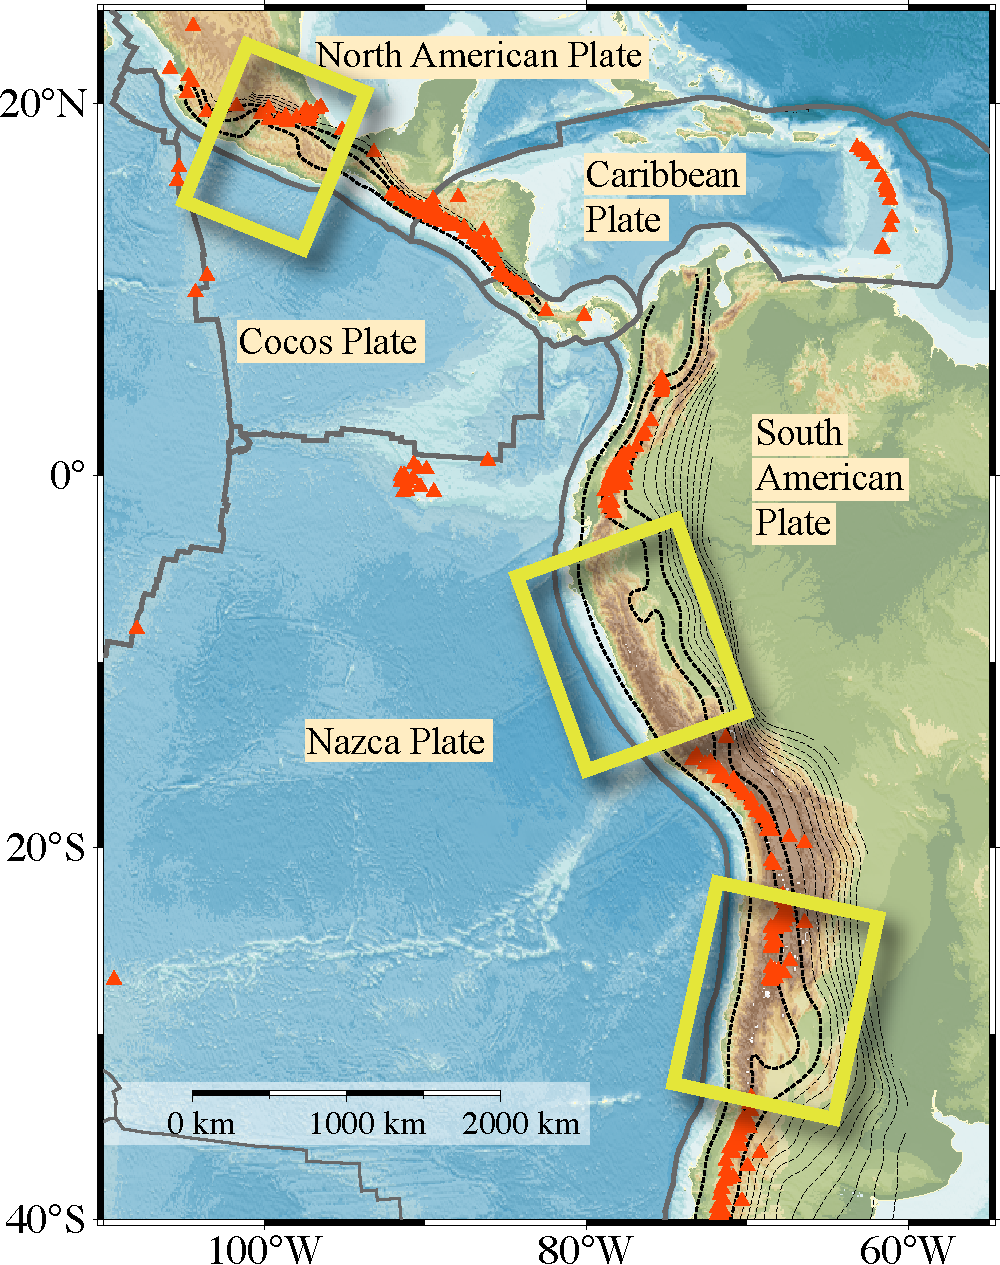
\includegraphics[width=6in]{flat_slab_vol_v1.pdf}
    \caption[研究區域板塊構造圖]{研究區域板塊構造圖,灰色實線為板塊邊界,資料來自\citet{bird2003updated},橘紅色三角形為火山分佈,資料來自\citet{venzke2013global},黑色虛線為每50公里深之板塊等深度線,其中50、100與150公里等深度線加粗,資料來自\citet{hayes2018slab2}。黃色框框圈起處為本研究所定義的平坦隱沒位置,由北到南分別位於墨西哥、秘魯與智利。
    }
    \label{fig::flat_slab_vol}
\end{figure*}

從物理的角度來看,造成隱沒板塊的傾角變化可以用力矩來解釋(\citealp{stevenson1977angle}),見圖\ref{fig::Torque}。
施加於隱沒板塊上的兩個轉動力矩分別為重力力矩(gravity torque)與動水壓力力矩(hydrodynamic pressure torque)(\citealp{McKenzie1969})。

重力力矩主要來自隱沒板塊與周遭地函的密度差。
同\ref{背景}所述,該密度差同時有化學與溫度上的影響: 玄武岩相變導致地殼密度增大,此為化學上之影響; 同時隱沒板塊溫度相對地函較低,導致海洋岩石圈密度較地函大,此為溫度上之影響。
由於重力(gravity force)指向地心,在圖\ref{fig::Torque}中,若假設海溝為轉動支點(fulcrum),則該隱沒系統之海洋岩石圈上任一點的重力效應,皆會造成順時針方向上的轉動。
而動水壓力力矩來自隱沒板塊下地函與隱沒板塊上地函楔(mantle wedge)的動水壓力差。
圖\ref{fig::Torque}中綠色線段為隱沒系統中假想的流線(streamline)。
相對於隱沒板塊下方的地函,隱沒過程中地函楔側之速度變化大,導致速度梯度大,容易產生低壓環境。
隱沒板塊下方的地函相對速度變化小,壓力相對高壓。
而為了平衡壓力,高壓會往低壓流動,此現象所產生的加速度稱為動水壓力(壓力梯度力),該力會垂直於隱沒板塊,且若壓力差越大,則動水壓力越大。
同樣假設海溝為轉動支點,這裡定義隱沒板塊上每個點所承受的動水壓力正向方向為朝地函楔為正,於是其所產生的正向動水壓力力矩於圖\ref{fig::Torque}中為逆時針轉動。
該轉動現象在看似對隱沒板塊產生往上吸的影響,因此動水壓力力矩又可稱為吸力力矩(suction torque)(\citealp{tovish1978mantle}),而動水壓力又可稱為吸力(suction force)。

\begin{figure*}[ht!]
    \centering
    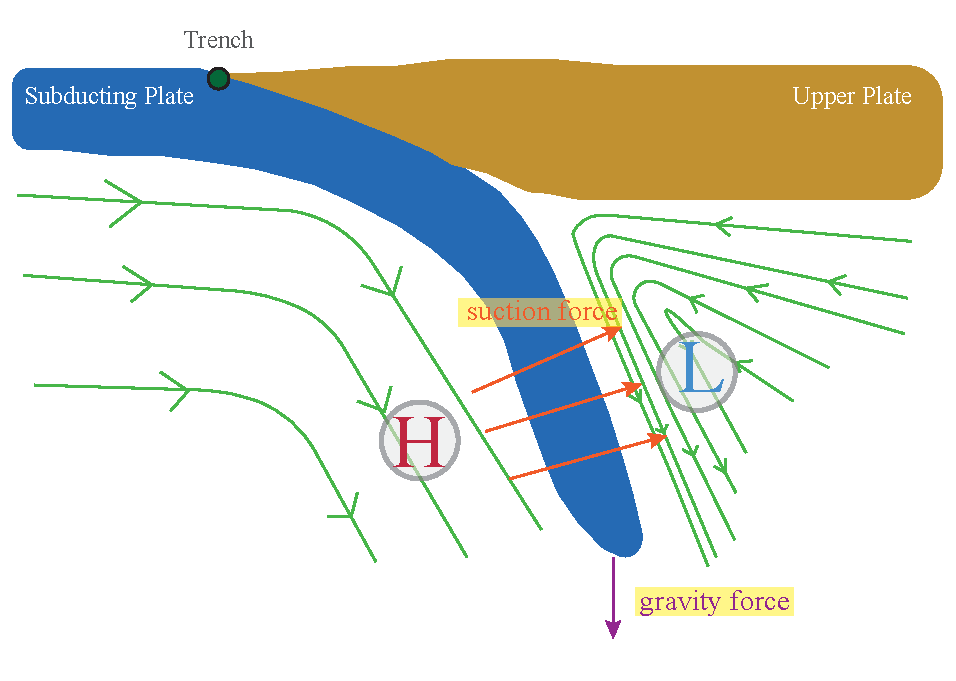
\includegraphics[width=6in]{torque_v3.pdf}
    \caption[隱沒系統中施加於隱沒板塊上的轉動力矩]{隱沒系統中施加於隱沒板塊上的轉動力矩,包含重力力矩與動水壓力力矩。綠色線為軟流圈(asthenosphere)中的假想流線,灰圓底紅字H代表高壓區,灰圓底藍字代表低壓區。假設海溝為支點,大於0之重力力矩在該系統中施予一順時針方向上的轉動,反之大於0之動水壓力力矩施予一逆時針方向上的轉動。
    }
    \label{fig::Torque}
\end{figure*}

隱沒系統的重力力矩直接與隱沒板塊有關,過去有不少數值模型改變隱沒板塊上的物質狀態形成平坦隱沒,例如,在隱沒板塊上放置一段增厚海洋地殼(\citealp{van2002role}; \citealp{Liu2016}; \citealp{Hu2016}等)、延後生成高密度的榴輝岩相或不生成榴輝岩相(\citealp{van2002role})、降低隱沒板塊整體密度(\citealp{Gerya2009})、設計斷掉的隱沒板塊(\citealp{Liu2016})等。
由於早期認為平坦隱沒的生成與隱沒板塊有直接關係,因此過去的數值模型研究在這方面已經相當豐富。

動水壓力力矩所牽扯到之因素較難約束,也較為複雜,例如上覆板塊的厚度、溫度、強度(strength)、受力狀態等,以及地函中的黏滯度(viscosity)、板塊聚合速率(convergent rate)、岩漿庫(magma chamber)位置與大小等,都有可能是影響動水壓力力矩大小的原因。
過去數值模型研究中,試圖以多種模型設定探討隱沒系統中動水壓力力矩增加的可行性,包含克拉通(craton)的存在(\citealp{Manea2012Chile}; \citealp{Liu2016}; \citealp{Hu2016})、隱沒帶中脫水作用所產生的低黏滯度區域(\citealp{Manea2007})與上覆板塊的溫度構造(\citealp{Thermal2012})。

以下將一一介紹過去研究的成果與目前尚待釐清的問題。
\newpage
\section{平坦隱沒的數值模型}\label{平坦隱沒的數值模型}
\subsection{隱沒的洋脊或海洋高原存在爭議}\label{隱沒的洋脊或海洋高原存在爭議}
早期概念模型研究將平坦隱沒與隱沒的洋脊(oceanic ridge)或海洋高原(oceanic plateau)的時空關係相連結(\citealp{pilger1981plate}; \citealp{henderson1984mesozoic}; \citealp{Gutscher2000A}; \citealp{gutscher2002andean}),\citet{Gutscher2000A}利用地震分布與早期地震波層析成像勾勒出隱沒的印加高原(Inca Plateau)與納茲卡中洋脊(Nazca Ridge)現今地下構造位置,成功與祕魯平坦隱沒的位置相對應(見圖\ref{fig::Gutscher_2000_ridge})。
對此,\citet{Gutscher2000A}認為海洋地殼上海洋高原與洋脊的存在可能會導致總體密度較低、浮力較大,
如\ref{背景}節所述,主要造成板塊隱沒的驅動力是隱沒後海洋地殼上的榴輝岩。
榴輝岩的密度高於地函,因此隱沒板塊可以產生足夠大的板塊拉力(slab pull)。
相比之下,海洋地殼的玄武岩質密度低於地函,故與普通的海洋地殼相比,較厚的海洋地殼在還沒有相變成榴輝岩之前密度確實較低,因此在隱沒初期能造成低傾角隱沒發生。
冷又厚的海洋岩石圈額外提供較低溫環境,導致榴輝岩化作用時間較長,於是系統中高密度物質體積較周遭其餘隱沒板塊小,促使平坦隱沒生成。

\begin{figure*}[htp]
    \centering
    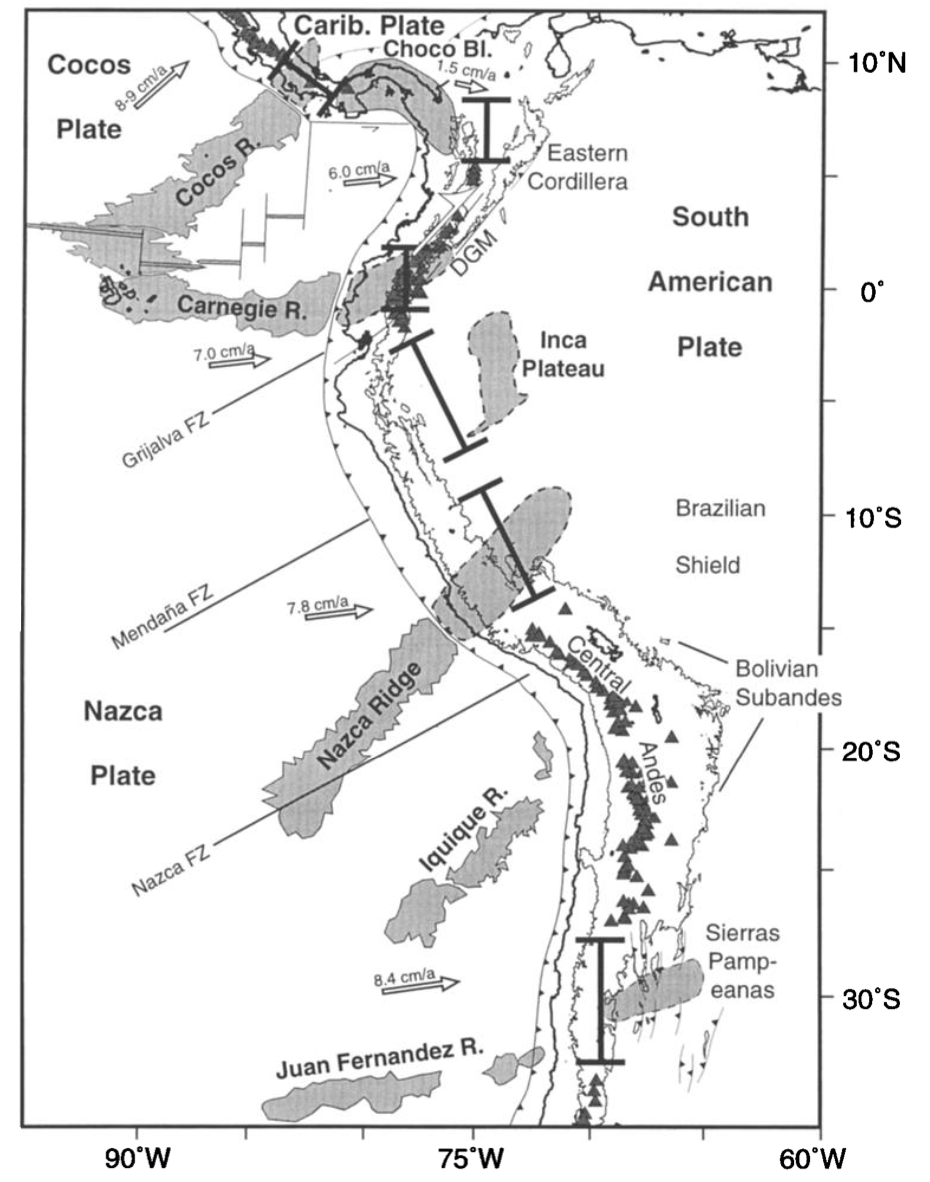
\includegraphics[width=6in]{Gutscher_2000_ridge.png}
    \caption[南美洲板塊構造圖,摘自\citet{Gutscher2000A}]{南美洲板塊構造圖,摘自\citet{Gutscher2000A}。粗黑線標出平坦隱沒段,灰色陰影區標示隱沒的海洋高原與洋脊,三角形為活動火山。板塊聚合速率由白色箭頭標出,參考自\citet{demets1990current}。
    }
    \label{fig::Gutscher_2000_ridge}
\end{figure*}

最早的平坦隱沒數值模型為\citet{van2002role} (見圖\ref{fig::van2002}),其利用二維尤拉笛卡爾座標熱化學數值模型,在海洋地殼上方增加一寬400公里、厚18公里的海洋地殼。
為了驗證\citet{Gutscher2000A}所提出的玄武岩相變延遲,\citet{van2002role}考慮成分隨時間的變化項,使用額外設定控制玄武岩相變成榴輝岩的延遲時間,為增厚的海洋地殼提供較大的浮力。
其結果表明若僅包含增厚的海洋地殼不足以形成平坦隱沒,需要同時有快速的板塊聚合速度才能觸發平坦隱沒的形成。
然而無論觀測上與實驗上對平坦隱沒的玄武岩相變延遲皆沒有太充足的證明。

\begin{figure*}[hb!]
    \centering
    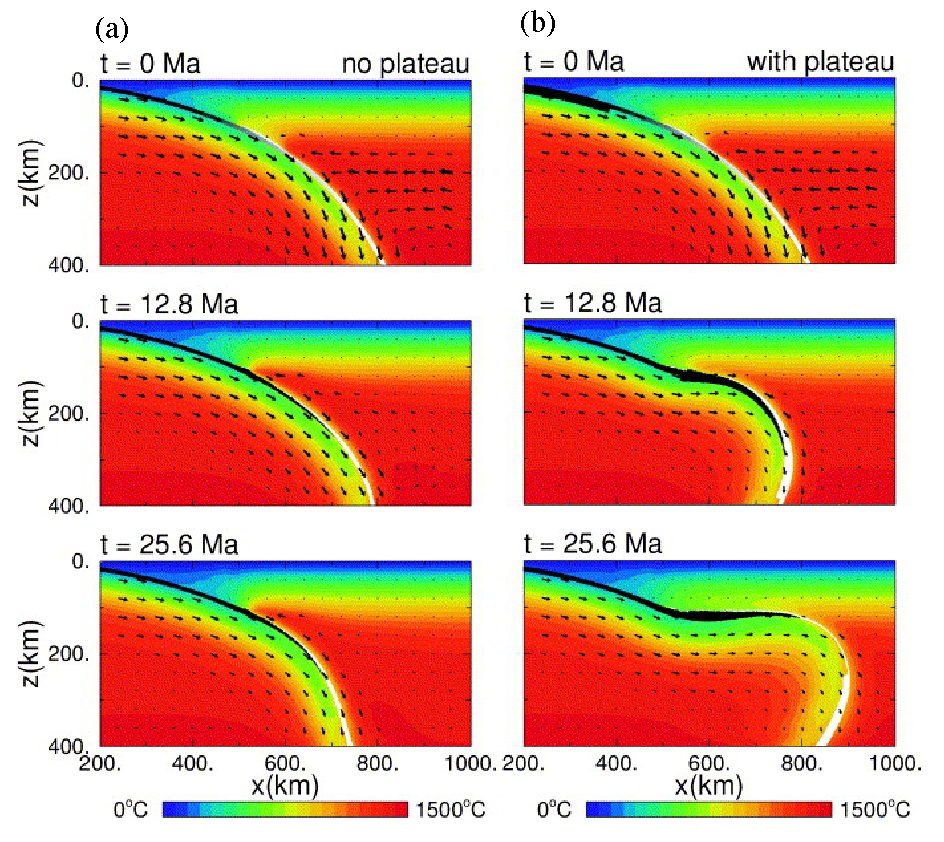
\includegraphics[width=6in]{van2002.pdf}
    \caption[正常的隱沒帶與包含海洋高原的隱沒帶隨模型時間變化,摘自\citet{van2002role}]{正常的隱沒帶(左)與包含海洋高原的隱沒帶(右)隨模型時間變化,摘自\citet{van2002role}。黑白區域繪出海洋地殼的化學成分從玄武岩(黑)到榴輝岩(白)的變化。水平軸為與海溝的距離,背景顏色為溫度。
    }
    \label{fig::van2002}
\end{figure*}

\citet{Gerya2009}使用二維尤拉笛卡爾座標模型(I2VIS)探討平坦隱沒帶與洋脊隱沒的關係,該模型包含脫水作用、部分熔融與地表高程變化。
為了模擬納茲卡洋脊的存在,模型中隱沒板塊上存在一200公里寬、18公里厚的玄武岩洋脊隱沒進入上覆板塊之下(見圖\ref{fig::Gerya2009})。
模型結果顯示平坦隱沒的形成與洋脊的存在與否無關,只要是密度異常低的海洋岩石圈(見圖\ref{fig::Gerya2009}a)皆有利於其形成。
並且,洋脊的存在與岩漿作用是否活躍也無關,當平坦隱沒存在,高溫的地函楔被隱沒板塊閉合,岩漿活動大量減少,有別於在相同情況下沒有平坦隱沒的隱沒帶(見圖\ref{fig::Gerya2009}b)。
值得一提的是,該模型並沒有考慮玄武岩至榴輝岩的相變過程,平坦隱沒在地殼密度低的情況下發育。

\begin{figure*}[ht!]
    \centering
    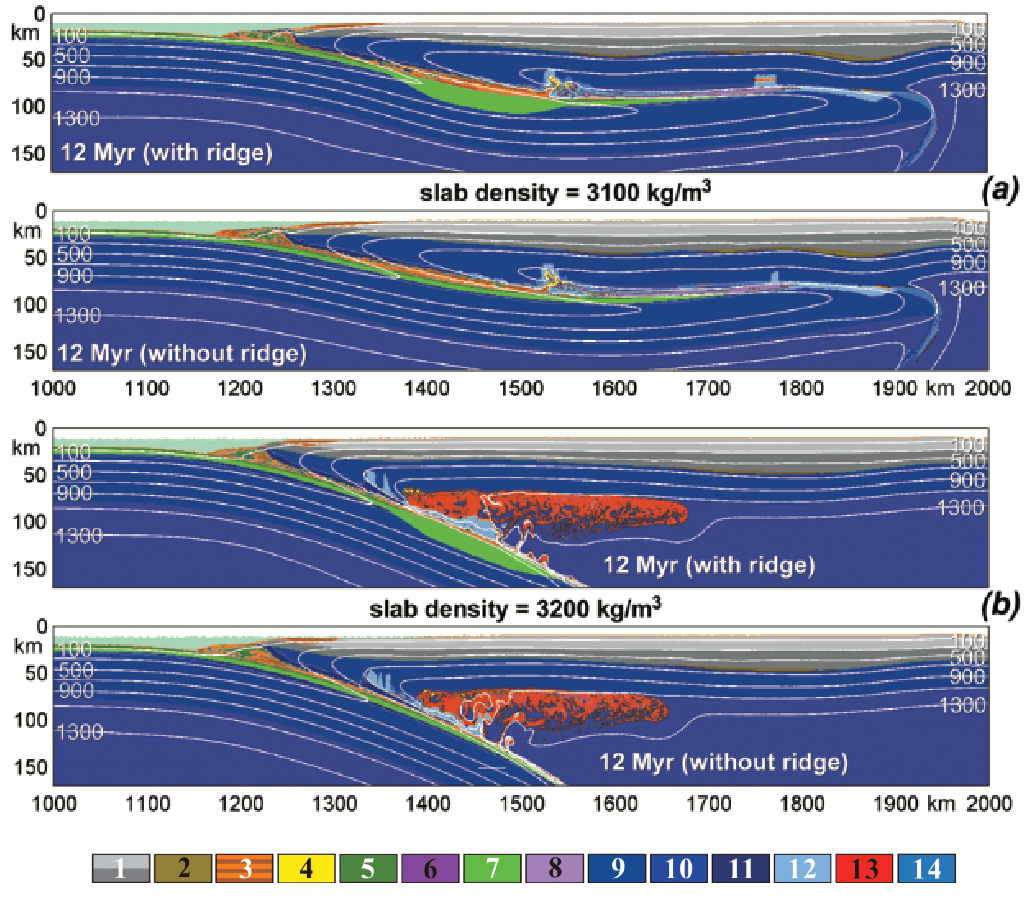
\includegraphics[width=6in]{Gerya_final.pdf}
    \caption[\citet{Gerya2009}平坦隱沒模型結果]{\citet{Gerya2009}中平坦隱沒模型於第12個百萬年的結果。圖組(a)與圖組(b)分別為隱沒海洋地函岩石圈密度為3100 kgm$^{-3}$與3300 kgm$^{-3}$的結果。(a)上圖與(b)上圖為包含洋脊隱沒的模型,(a)(b)下圖為不包含洋脊的模型,圖中白線為等溫線。其中,顏色代表不同岩相: 1、2 = 大陸地殼、3、4 = 沉積物、5、6 = 玄武岩、7、8 = 輝長岩、9、10 = 無水地函、11 = 蛇紋岩、12、13、14 = 含水地函。
    }
    \label{fig::Gerya2009}
\end{figure*}

\citet{Liu2016}利用二維任意拉格朗日-尤拉模型(SOPALE)討論過去拉臘米造山運動(Laramide orogeny)時期($\sim$80–50百萬年前)法拉龍板塊(Farallon plate)發生的平坦隱沒事件。
模型的隱沒板塊上設定一段400公里寬的海洋高原,包含18公里厚的增厚玄武岩海洋地殼與36公里厚的斜輝橄欖岩(harzburgite)地函岩石圈。
該模型也假設海洋高原上的玄武岩並不會發生榴輝岩相變,並且斜輝橄欖岩地函岩石圈密度比周遭地函低100 kg$\cdot$m$^{-3}$。
研究結果表明增厚海洋高原與快速的聚合板塊是平坦隱沒發育的必要條件。
模型中同樣沒有考慮玄武岩至榴輝岩相變過程。

上述研究中,將模型加入增厚海洋地殼的結果雖然都能讓平坦隱沒發育,但皆存在兩個問題。
第一,上述文獻中所有模型皆是二維模型,這意味著在第三維上有無限延伸的增厚海洋地殼,於是,增厚洋殼能在二維假設下提供足夠大的浮力,然而現實中增厚洋殼能造成的浮力效應應遠小於二維模型中的結果。
\citet{florez2019impact}在三維模型中證明了這一點,他們的研究結果表明若將現在自然界中最大的洋脊隱沒進入地函中,其所提供的浮力也只會造成海洋板塊傾角減少原先的10度。
除此之外,浮力效應的量值是另一個潛在問題。
增厚的海洋地殼之所以能為隱沒板塊提供浮力,是因玄武岩的密度小於橄欖岩地函。
隱沒過程中,儘管玄武岩與地函橄欖岩的密度差不變,增厚的海洋地殼相對於正常海洋地殼擁有更大體積的低密度物質,因此能產生更大的浮力。
不過一旦玄武岩相變至榴輝岩相,大體積榴輝岩所造成的重力效應將會導致隱沒板塊重力力矩急劇增大,反而會抑制平坦隱沒的發育。
這緊接著點出後續問題。
第二,過去研究針對玄武岩至榴輝岩相變過程並沒有完善的解釋,\citet{van2002role}所使用的相變延遲現象無法用實驗所證明,而剩餘研究皆沒有考慮此相變過程。
對此,上述對重力力矩減少的原因事實上難以與自然界的觀測吻合。


\subsection{實現數值模型中增加的地函動水壓力力矩}
\citet{tovish1978mantle}計算隱沒帶中的角流(corner flow)指出非牛頓流體的地函可以產生極大的地函流吸力(mantle flow suction force),此時動水壓力力矩足夠抵抗重力力矩,形成平坦隱沒。
不過正如\ref{背景}節所述,不同於重力力矩直接與隱沒板塊物理特徵有關,隱沒系統中能夠影響動水壓力力矩的因素難以被量化與控制,因此過去討論動水壓力力矩的數值模型研究較少。

\citet{Manea2007}使用二維模型CitcomS研究隱沒帶中脫水作用、地函黏滯度與動水壓力對隱沒板塊幾何的影響。
模型的地函楔中假設隱沒板塊脫水作用會產生一近似梯型低黏滯度區,詳見圖\ref{fig::Manea2007}。
他們改變圖\ref{fig::Manea2007}中橘紅色區域的黏滯度,發現較低的黏滯度可以增加地函楔中的壓力,導致板塊兩側的壓力差減少,大幅度減少隱沒系統的地函流吸力。
該研究指出過去\citet{tovish1978mantle}的解析解研究並沒有考慮隱沒帶中的脫水作用影響,這意味著過去計算隱沒板塊力矩時,很可能高估地函吸力的量值。
%數值模型雖然可以透過測試地函黏滯度量值獲得平坦隱沒模型,然而黏滯度量值大範圍的不確定性難以證明模型的真實性。

\begin{figure*}[ht!]
    \centering
    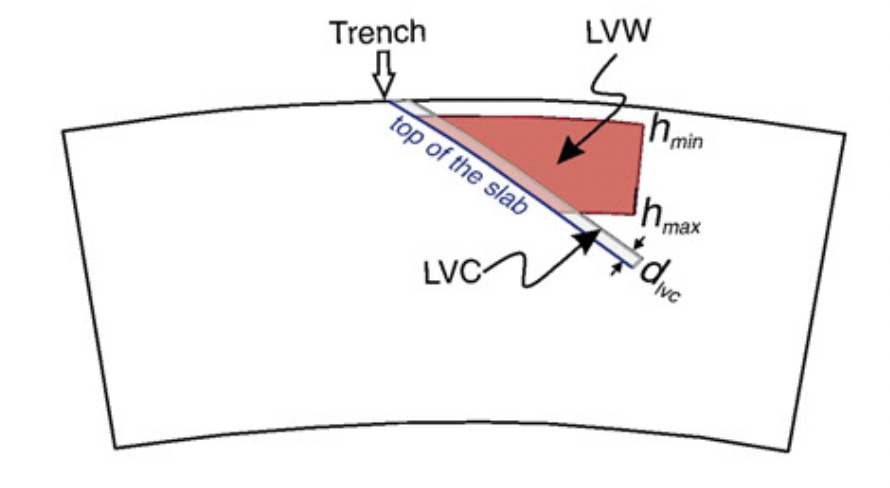
\includegraphics[width=3in]{Manea2007.png}
    \caption[\citet{Manea2007}模型中所設定的低黏滯度近似梯形區與低黏滯度通道區域]{\citet{Manea2007}模型中所設定的低黏滯度近似梯形區(LVW, low viscosity wedge)與低黏滯度通道(LVC, low viscosity channel)區域,表示隱沒帶的脫水作用對地函楔造成的影響。其中h$_{min}$、h$_{max}$、d$_{lvc}$皆為模型中可調整的參數,用以控制低黏滯度近似梯形區與低黏滯度通道的範圍與深度。}
    \label{fig::Manea2007}
\end{figure*}

\citet{Thermal2012}利用包含牛頓流體(diffusion creep)與非牛頓流體(dislocation creep)的複合流變學不可壓縮流二維模型,討論上覆板塊的溫度構造與平坦隱沒的關係,模型中海溝位置不隨時間改變。
他們的結果認為冷硬的大陸岩石圈可以促使隱沒板塊角度變低,同時他們使用解析解的方式計算模型中重力力矩與動水壓力力矩的大小。
該研究結論支持平坦隱沒不是一個穩態(steady-state)狀態,平坦隱沒只有在隱沒作用初期、隱沒板塊長度不到400公里時會出現。
不過這與現生的平坦隱沒形成時間抵觸,無論是智利、秘魯或墨西哥的平坦隱沒都不是隱沒初期的構造,三個地區的隱沒帶已經隱沒超過180 Ma(\citealp{Schellart2021}),然而根據火成岩研究(\citealp{Manea2017}),平坦隱沒事件的發生時間在墨西哥為15 Ma左右,而秘魯與智利的平坦隱沒事件發生在6 Ma(\citealp{chen2019southward}; \citealp{hu2021southward}),亦即這些平坦隱沒都是自正常的隱沒角度逐漸演化成平坦隱沒。

\citet{o2009subduction}利用有限元素法模型計算增厚大陸岩石圈對地函楔角流(mantle wedge corner flow)的影響,進而計算地函楔動水壓力的大小。
他們的結果顯示若大陸岩石圈具有250公里厚且寬度200公里的山根(root)時,地函楔中的角流降低,動水壓力力矩可增加至原先無山根模型的四倍。
儘管他們的模型研究並沒有包含平坦隱沒,但大陸岩石圈山根影響動水壓力力矩的概念成功開啟往後動水壓力力矩的數值模型研究,為後續平坦隱沒數值模型的研究提供新的方向。

\citet{Manea2012Chile}利用三維模型模擬過去30個百萬年來智利區域的隱沒帶動態行為,邊界條件與\citet{Thermal2012}幾乎相同。
模型開始先是普通的隱沒帶模型,在隱沒帶發育成熟後,額外施加一段邊界條件強迫智利海溝後撤,他們發現海溝後撤能夠施加給隱沒板塊的地函流吸力,不過該吸力量值不足以讓巨大厚重的海洋板塊變平坦。
爾後他們效仿\citet{o2009subduction}的模型設計,嘗試將南美洲大陸數個古老克拉通(craton)地塊加入模型中。
利用改變上覆板塊溫度梯度,讓模型的上覆板塊厚度增厚,此初始設定代表冷硬的克拉通構造,該地質構造成功讓地函楔角流下降,隱沒帶系統的動力壓力增加,平坦隱沒得以順利形成,見圖\ref{fig::Manea 2012}。
因此他們得出的結論是需要同時有海溝後撤與克拉通的存在才會觸發平坦隱沒,這是首次在不更改隱沒板塊狀態、僅利用增加動水壓力產生的平坦隱沒模型。
他們的模型中沒有考慮地殼與地函的密度差,也沒有考慮任何相變過程。
隨後\citet{Liu2016}效仿同樣的概念,將過去普遍認為存在於北美岩石圈西部下方的科羅拉多高原山根(Colorado Plateau)放入模型中,模擬法拉龍板塊平坦隱沒演化。
然而他們的研究表示克拉通或山根的存在只是加快平坦隱沒的形成,但真正觸發平坦隱沒的機制是增厚且沒有榴輝岩相變的海洋地殼,亦即動水壓力力矩對隱沒帶的影響並不大。
\begin{figure*}[ht!]
    \centering
    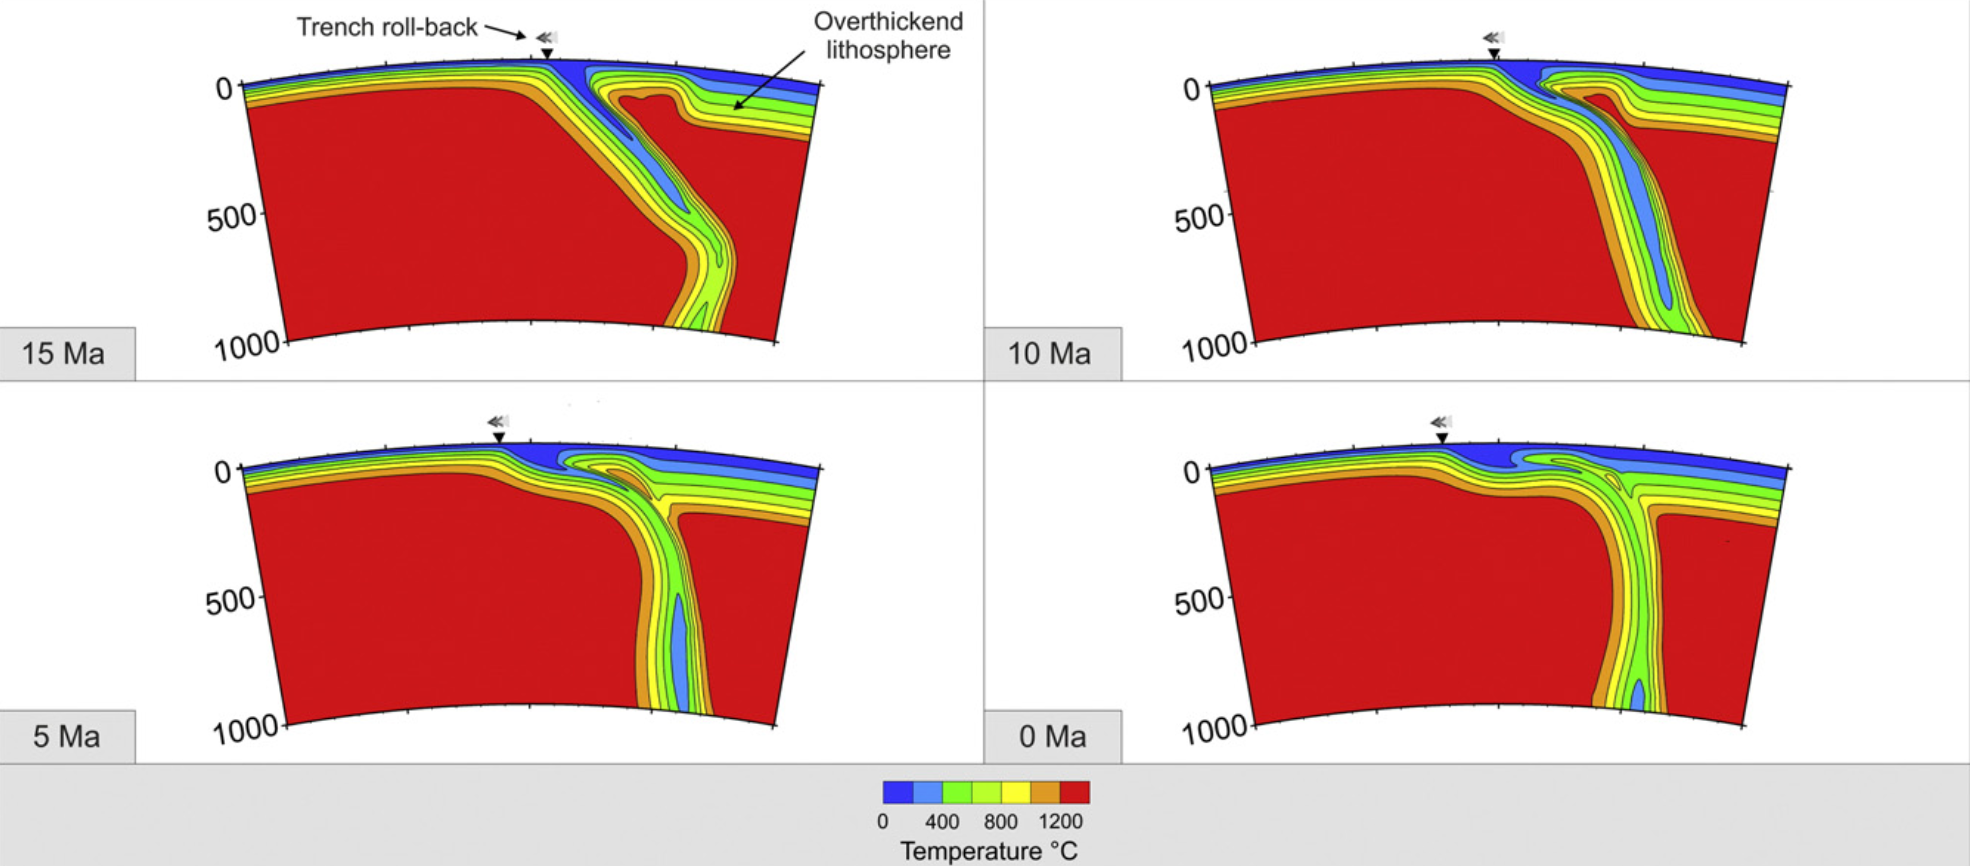
\includegraphics[width=6in]{Manea 2012.png}
    \caption[\citet{Manea2012Chile}中的智利平坦隱沒模型]{\citet{Manea2012Chile}中的智利平坦隱沒模型,模型中同時加入海溝後撤邊界條件與增厚大陸岩石圈可以讓平坦隱沒發育。模型背景顏色為溫度。
    }
    \label{fig::Manea 2012}
\end{figure*}

\citet{Hu2016}重複與\citet{Manea2012Chile}同樣的實驗,使用三維模型CitcomS模擬阿他加馬海溝(Atacama Trench, or Peru–Chile Trench)於45個百萬年以來隱沒帶的演化。
這次他們將觀測資料當作模型邊界條件,逐一分析海溝後撤、海洋高原隱沒與克拉通山根的存在對模型的影響,用以探討影響平坦隱沒形成的關鍵原因。
模型加入克拉通後,隱沒板塊傾角有降低的趨勢,不過克拉通的影響不足以形成平坦隱沒,僅能視為低傾角隱沒。
隨後模型加入隱沒的海洋高原,隱沒傾角在區域(local)上顯著降低,表明隱沒的海洋高原才是平坦隱沒發育的主因。
故動水壓力力矩與重力力矩對平坦隱沒發育的角色仍然存在分歧。

\section{研究動機}\label{研究動機}
最簡單直接的平坦隱沒概念模型可以透過改變隱沒系統的重力力矩達成,尤其是早期的隱沒洋脊理論,然而過去動力學數值模型研究針對玄武岩至榴輝岩相變過程並沒有完善的物理機制解釋。
相較於隱沒帶中重力力矩的直觀性,動水壓力力矩增大的條件與其對隱沒帶造成的影響較難以用單一的地質構造或特性約束。
近年來地球動力學數值模型除了為地球內部構造提供物理約束外,也開始量化各種自然現象對岩石造成的物理特性改變,包含岩漿作用與脫水作用等。
尤其動水壓力力矩對隱沒系統的影響還沒有完全成熟,而這些較為複雜的地球內部作用或許可以為動水壓力力矩與隱沒帶構造的關係提供額外資訊。

過去研究還有另一個隱性問題,上述所有數值模型皆是模擬南美洲區域的隱沒帶。
對本研究所定義的平坦隱沒(詳見\ref{平坦隱沒定義}節),目前世界上只有墨西哥、秘魯與智利有平坦隱沒的現象。
而過去研究皆是以南美洲的秘魯與智利的平坦隱沒當作模型藍本,少部分考量法拉龍板塊的平坦隱沒事件,值得一提的是,目前尚未有任何墨西哥平坦隱沒的數值模型被提出。
在墨西哥,隱沒板塊上沒有任何隱沒海脊的紀錄,上覆板塊也沒有任何克拉通存在的證據,因此墨西哥的平坦隱沒確切原因更是沒有明確方向。

本研究將著重在探討動水壓力力矩在哪些環境下會發生改變,並且在考慮玄武岩至榴輝岩相變的過程下模擬平坦隱沒的發育,此外,本研究期待能利用數值模擬墨西哥平坦隱沒,填補過去尚未成熟的平坦隱沒機制。
接下來會針對各個平坦隱沒區域的觀測資料進行文獻回顧,包含納茲卡隱沒帶的秘魯、智利平坦隱沒區域以及科克斯隱沒帶上的墨西哥平坦隱沒。


\section{秘魯與智利隱沒帶的地球物理觀測}\label{秘魯與智利隱沒帶地球物理觀測}
\citet{barazangi1976}利用南美洲區域震源位置資料判斷秘魯與智利下方的隱沒板塊處於水平狀態,由於南美洲沿岸的地震事件數目多,可藉由垂直海溝剖面的班尼奧夫帶(Benioff seismic zone)很好的勾勒出隱沒板塊的角度與形狀。

不過秘魯與智利區域的地震測站並不多,導致過去並沒有太多地區性的地震層析成像研究。
\citet{Ma2014}是第一個針對秘魯區域的速度構造研究,他們的結果展示秘魯平坦隱沒最南段的表面波層析成像(surface wave tomography)。
隨後\citet{Ma2015}利用接收函數判斷秘魯平坦隱沒上方的莫荷面(Moho),再配合\citet{Ma2014}的層析成像結果,獲得秘魯平坦隱沒板塊上的構造,如圖\ref{fig::Peru_tomography}。
隱沒板塊的平坦段約在距海溝100公里處,深度落在80-100公里之間,並且平坦段並非呈現水平,而是有上凹又下凹的構造,平坦段長度大約350公里。
他們的結果表明秘魯的莫荷面與隱沒板塊的深度側向變化非常接近,可能暗示著該區域有強烈的板塊間吸力。
此外,他們觀察到在平坦隱沒距海溝較近處有高速的地函岩石圈(mantle lithosphere),V$_S$可達到4.5 km/s,該研究解釋為乾冷的岩石圈,見\ref{fig::Peru_tomography}下圖深橘色區段。
直到距離海溝350公里後,快速的地函岩石圈V$_S$降低成4.2-4.3 km/s左右,該速度是正常地函岩石圈的速度,他們解釋,可能是隱沒板塊上的物質直到距離海溝350公里後才發生脫水。

\begin{figure*}[ht!]
    \centering
    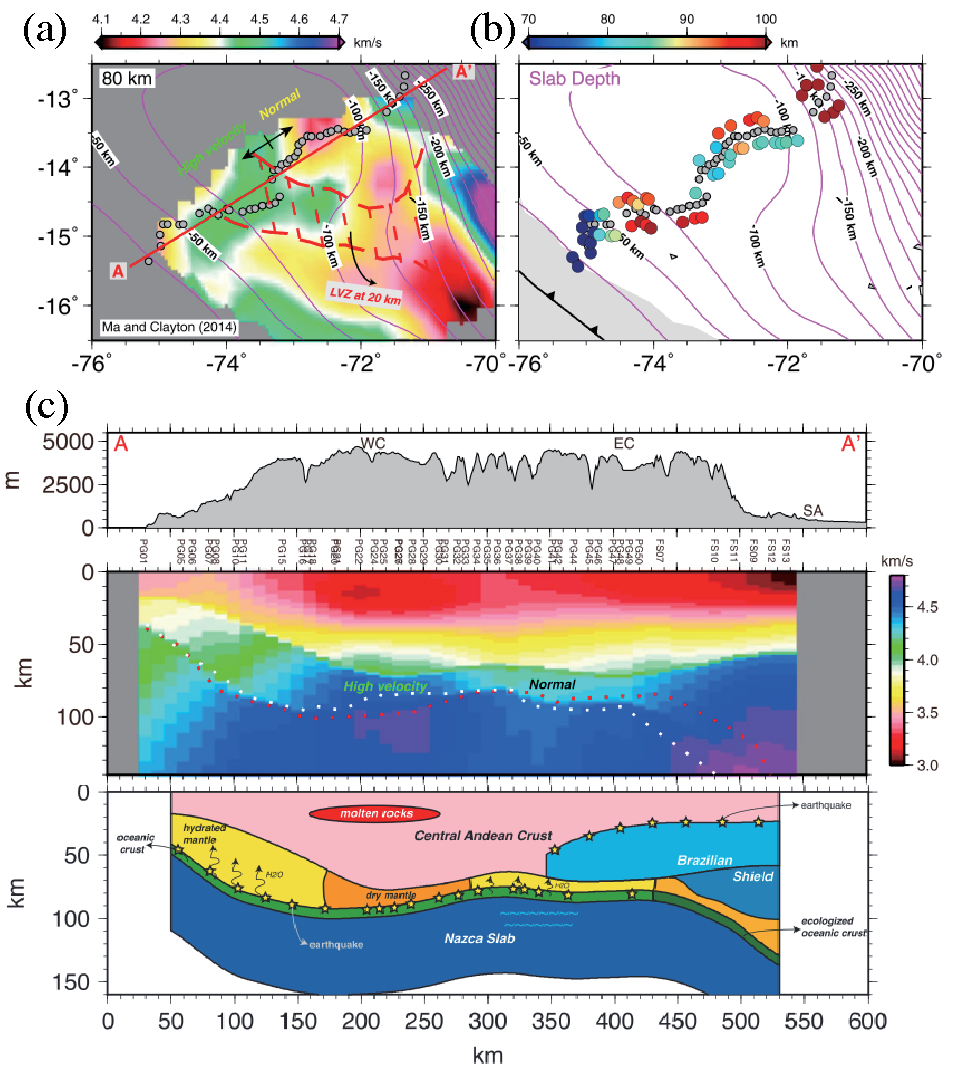
\includegraphics[width=5in]{Peru_tomography.pdf}
    \caption[秘魯平坦隱沒南段地震學研究結果與解釋圖,摘自\citet{Ma2015}]{秘魯平坦隱沒南段地震學研究結果與解釋圖,摘自\citet{Ma2015}。(a)深度80公里的V$_{SV}$速度構造,來自\citet{Ma2014}。圖中左上方標示高速地函岩石圈與正常地函岩石圈的分界。紅色虛線標示出於20公里深的低速帶範圍,該低速帶被解釋為熔融區。粉紅色線為板塊等深度線。紅色實線為圖(C)中AA'剖面位置。灰色點為該研究所使用的側站位置。(b)板塊等深度圖,各顏色點為接收函數轉換波的地殼入射點,顏色代表不同深度。灰色點為該研究所使用的側站位置。(c)最上圖為AA'剖面地形,中圖為AA'剖面V$_{SV}$速度構造圖,白色點與紅色點分別為接收函數於西北地震事件群與東南地震事件群所獲得之板塊深度。最下方為AA'剖面結構卡通圖,大陸與海洋莫荷面深度來自圖(b)中的結果。
    }
    \label{fig::Peru_tomography}
\end{figure*}

\citet{Marot2014}利用三維區域地震層析成像與衰減模型討論了圖\ref{fig::Chile_geology_profile}中智利平坦隱沒與智利南段正常隱沒帶的構造差異。圖\ref{fig::Chile_geology_profile}c、圖\ref{fig::Chile_geology_profile}d分別為平坦與正常的隱沒帶地震事件剖面,可見在平坦隱沒板塊區域的地震事件遠多於正常的隱沒板塊區域。他們的結果顯示平坦段在深度25、50與70公里處各有一段低速帶,如圖\ref{fig::Chile_tomography},在透過熱模型與速度對比後,他們認為低速帶可能是板塊脫水區,這導致蛇紋岩化橄欖岩在局部生成,正常的隱沒板塊段同樣也有類似的速度構造結果。
經過速度與熱構造比對後,他們判斷脫水區的蛇紋岩化橄欖岩比例約落在20$\%$。
然而在板塊到達70公里深後,平坦隱沒剖面的地函岩石圈速度快速,岩石V$_P$約8.0-8.5 km/s,V$_S$約4.5-4.8 km/s,並有相對較低的V$_P$/V$_S$比值(1.75-1.77),反映該高速區可能是較低的溫度所造成,暗示著冷硬的地函岩石圈。
他們認為平坦部分最有可能由非常乾燥的地函組成,有部分的榴輝岩化,並且密度可達3500-3600 kgm$^{-3}$。
深度90-100公里處的蛇紋岩化橄欖岩約有7$\%$的含水量,依然是乾燥的環境。
此外,該研究並沒有在平坦隱沒板塊段上發現任何增厚的紀錄,他們的隱沒板塊厚度最厚處不會超過10公里,並沒有看到胡安斐南德斯洋脊(Juan Fernández Ridge)的構造。

\begin{figure*}[ht!]
    \centering
    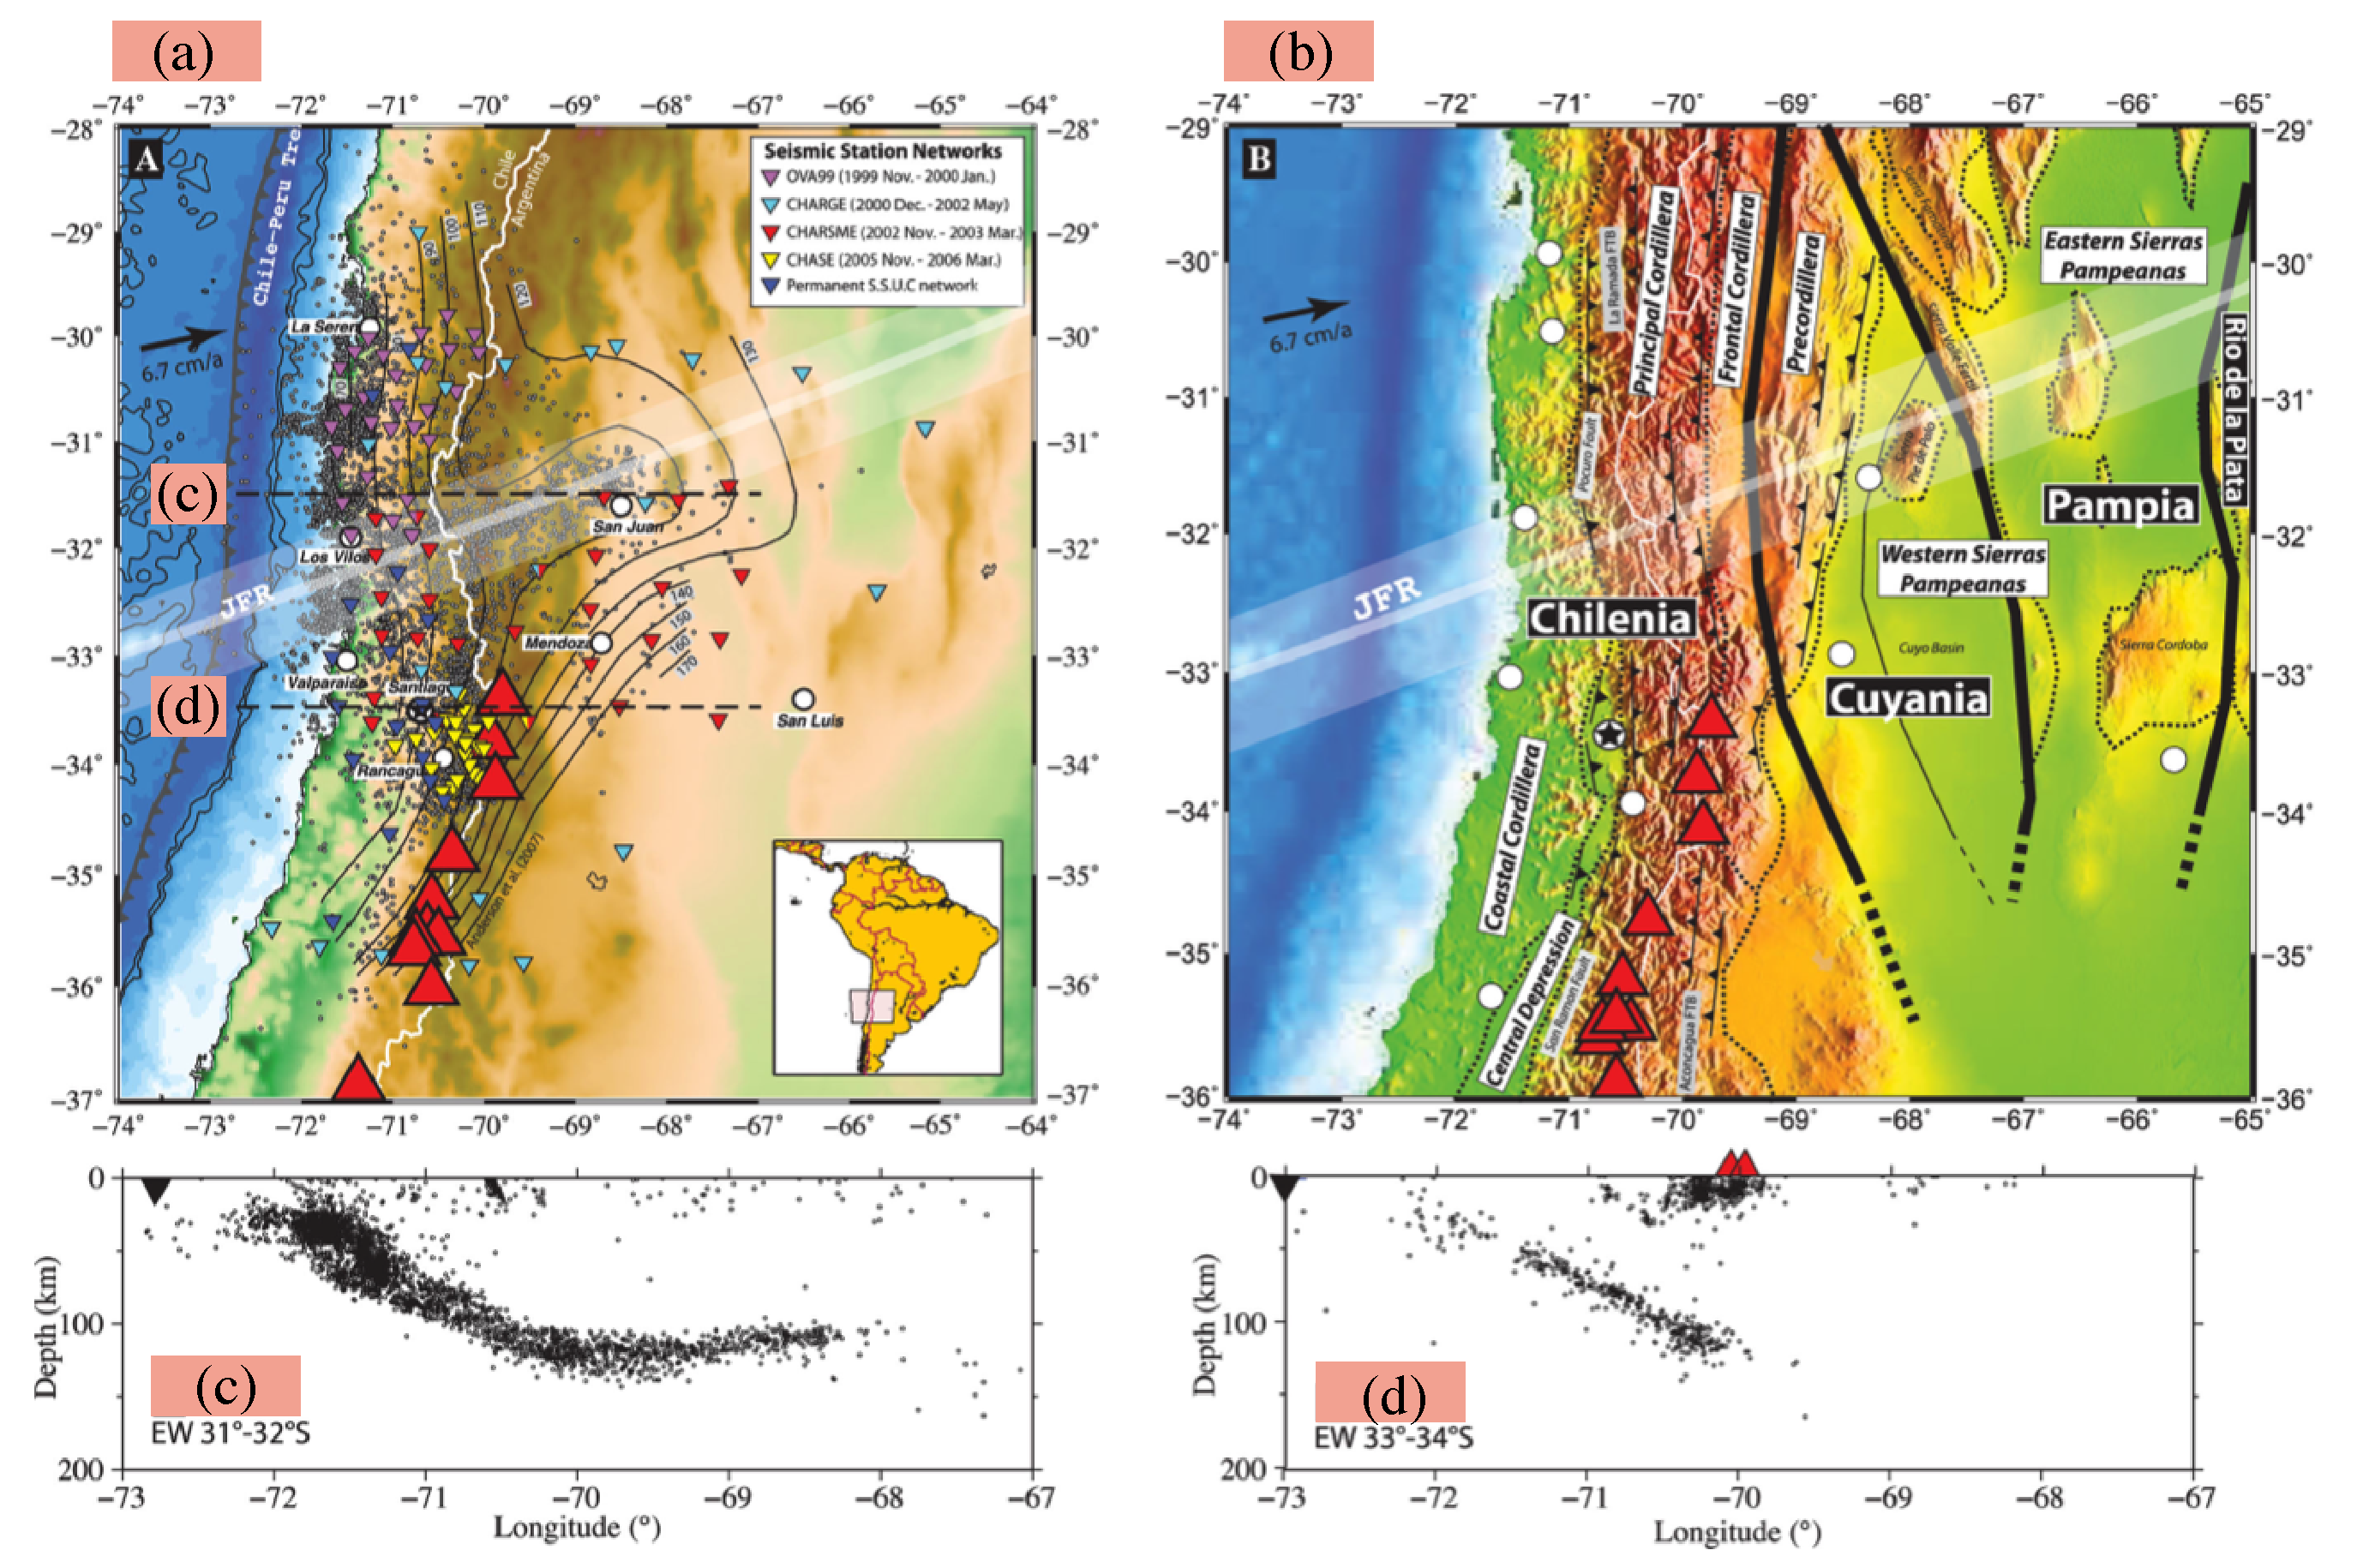
\includegraphics[width=5in]{Chile_geology_profile.pdf}
    \caption[智利中部和阿根廷西部的地質構造與地震活動度背景圖,摘自\citet{Marot2014}]{智利中部和阿根廷西部的地質構造與地震活動度背景圖,摘自\citet{Marot2014}。(a)納茲卡板塊隱沒進入南美板塊的海溝由帶三角形的黑線標出。臨時地震網以倒三角形表示,地震分佈由灰點標出,紅色正三角形為活火山分佈,隱沒板塊等深度線資料來自\citet{anderson2007geometry}。白線為智利與阿根廷的國界,白色圈圈為主要城市,其中黑色星星為智利首都聖地牙哥(Santiago)。灰線與灰透明底為推斷的胡安斐南德斯洋脊隱沒路徑與寬度,插圖為宏觀地圖,兩條黑色虛線為該研究中所觀測的剖面,分別為南緯31.5度(平坦隱沒區)與南緯33.5度(正常隱沒區)。(b)粗黑線標示主要地質縫合帶,帶三角形的黑細線為La Ramada與Aconcagua斷層,白色圈圈為主要城市,紅色正三角形為活火山分佈。(c)(d)為圖(a)中的剖面,黑色點顯示平坦板塊與正常板塊區域的地震活動,倒黑色三角形是海溝位置,紅色三角形是活火山。
    }
    \label{fig::Chile_geology_profile}
\end{figure*}

\begin{figure*}[ht!]
    \centering
    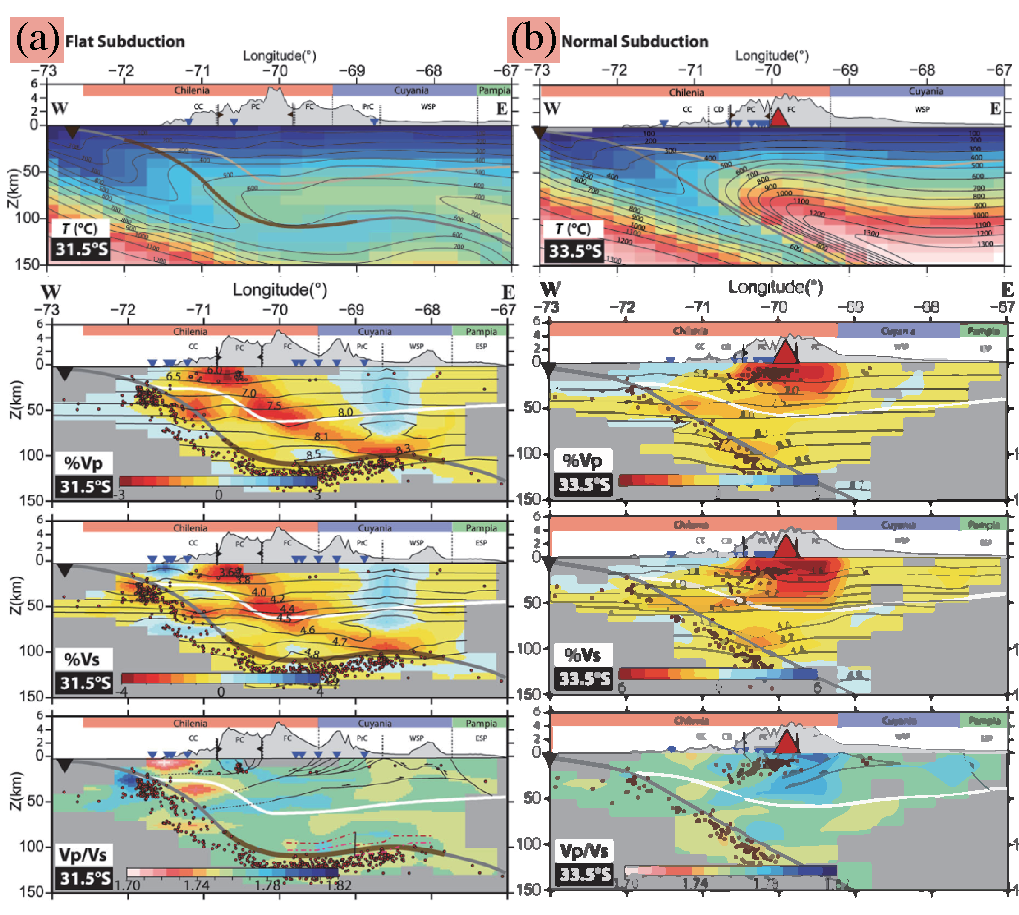
\includegraphics[width=6in]{Chile_tomography.pdf}
    \caption[智利中部和阿根廷西部的熱模型與速度構造剖面,摘自\citet{Marot2014}]{智利中部和阿根廷西部的熱模型與速度構造剖面,摘自\citet{Marot2014}。由上至下為熱構造剖面、V$_P$速度變化、V$_S$速度變化與V$_P$/V$_S$比值,速度構造剖面中的等高線為絕對地震速度。紅點代表該研究地震層析成像所選用的地震事件。白線為莫荷面,灰線為隱沒板塊頂部。(a)為圖\ref{fig::Chile_geology_profile}a中的C剖面。(b)為圖\ref{fig::Chile_geology_profile}a中的D剖面。
    }
    \label{fig::Chile_tomography}
\end{figure*}

總體而言,秘魯與智利平坦隱沒區的速度構造剖面同樣具有乾冷的地函岩石圈,且隱沒帶中平坦段的脫水作用不顯著。
\newpage
\section{墨西哥隱沒帶地球物理觀測}\label{墨西哥隱沒帶地球物理觀測}
相較於南美洲,墨西哥的平坦隱沒較晚才被發現。墨西哥平坦隱沒區域位在科克斯板塊與北美板塊(North American Plate)聚合處,該地區的地震活動度較低,並且地震事件集中在距海溝100公里以內、深度20公里的範圍,因此過去難以利用地震事件隨深度分佈描繪出科克斯板塊隱沒帶的幾何形狀。

\citet{pardo1995}藉由當地地震目錄重新定位震源判斷在墨西哥中部的板塊交界處下方有平坦隱沒存在,為最早對墨西哥區域的平坦隱沒研究。
\citet{PerezCampos2008}使用接收函數方法(receiver function method)得到清晰的平坦隱沒板塊特徵,如圖\ref{fig::receiverfunction2008}。
該剖面北部顯示大陸地殼與地函之間的莫荷面,見\ref{fig::receiverfunction2008}上圖的接收函數影像,南部則些微顯示一個水平介面,如圖\ref{fig::receiverfunction2008}左下,深度落在40-50公里之間,平坦段長度約100-200公里。
有別於南美洲區域的平坦隱沒,墨西哥的平坦隱沒深度幾乎與地殼貼齊,他們起初推測長達超過100公里的板塊交界面具有強大摩擦力,理論上應有強耦合特性,亦即該地區應該容易累積大量應力產生多起地震事件。
然而正如前面所提到,墨西哥平坦隱沒段的地震活動度極低,在墨西哥平坦隱沒上方的格雷羅州擁有世界知名的格雷羅無震帶(Guerrero gap)。
GPS研究也支持該地區並不是強耦合板塊介面(\citealp{nieto2006latest})。
並且,墨西哥區域的平坦隱沒持續時間(15 Ma)比安地斯山脈平坦隱沒來得長(4-5 Ma),然而墨西哥平坦隱沒上方並沒有顯著的水平壓縮現象(\citealp{moran2007cenozoic})。
種種跡象表示墨西哥平坦隱沒區可能是弱耦合(weak coupling)的環境,與平坦隱沒的存在產生矛盾。
對此,板塊交界處需要有可行機制解釋該地區弱耦合現象。

\begin{figure*}[ht!]
    \centering
    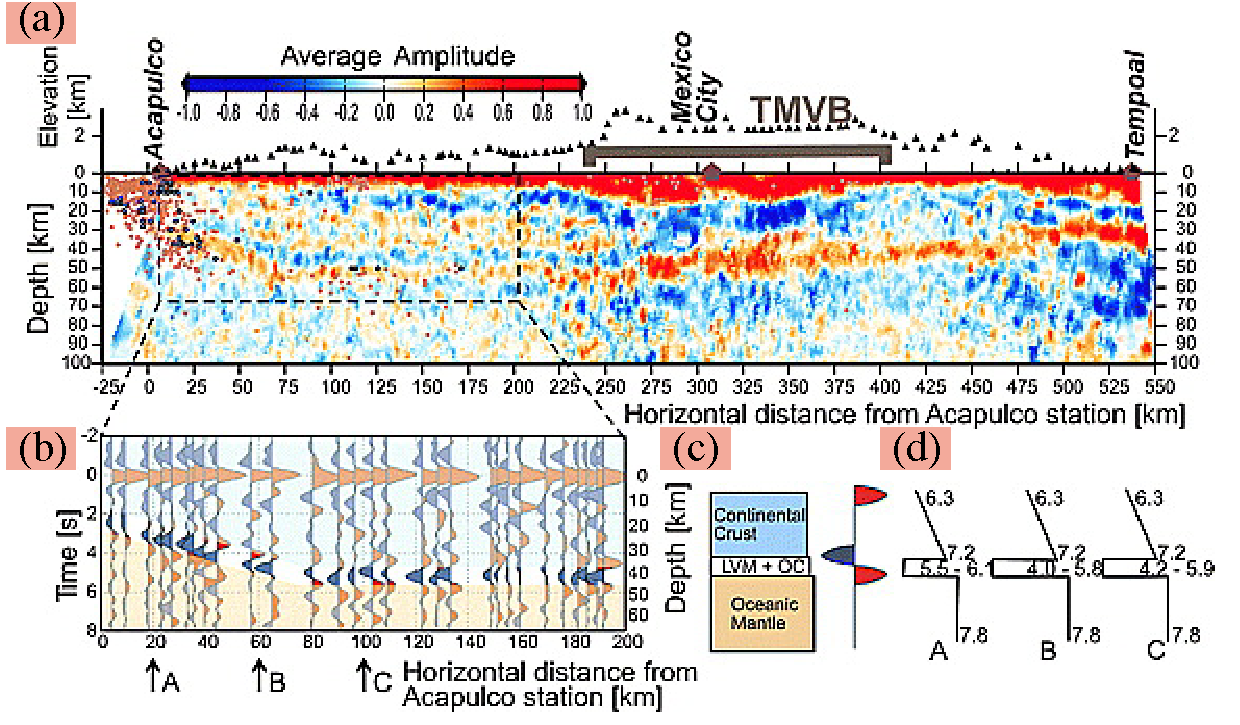
\includegraphics[width=6in]{2008receiverfunction.pdf}
    \caption[墨西哥平坦隱沒區域接收函數結果,摘自\citet{PerezCampos2008}]{墨西哥平坦隱沒區域接收函數結果,摘自\citet{PerezCampos2008}。
    (a)中黑色三角形表示測站沿剖面的位置,高程被放大10倍。
    粗棕色線表示跨墨西哥火山帶(TMVB, Trans-Mexican Volcanic Belt)的範圍。
    接收函數影像中標出沿剖面50公里範圍內的震源(粉紅色點來自SSN地震目錄,綠色點來自\citet{pardo1995}重新定位結果)位置。
    (b)顯示沿平坦隱沒板塊的一次遠震事件的接收函數。
    (c)說明了相應的模型(LVM (low velocity mantle) = 低速地函和 OC (oceanic crust) = 海洋地殼)。
    (d)根據左下圖接收函數模型中A、B和C位置上的P波速度模型。
    }
    \label{fig::receiverfunction2008}
\end{figure*}

\citet{PerezCampos2008}在平坦隱沒板塊段與大陸板塊交界處中,初步判斷有一約略10±3公里厚的低速帶,速度模型如圖\ref{fig::receiverfunction2008}右下。
他們推測該低速層很可能是弱耦合現象的主因。
\citet{Song2009}利用平坦隱沒上方地區性慢速滑移事件的轉換SP波進行波形模擬,確認該低速層厚度約3-5公里,並且其V$_S$速度約每秒2.0-2.7公里。
爾後\citet{Song2012SC}發現該低速區的地震非均向性傾角方向與隱沒板塊介面傾角方向有20±10$^{\circ}$的夾角,如圖\ref{fig::SCanisotorpy2012}所示,與S(葉理面)-C(剪切面)糜棱岩中發育的葉理方向一致,再藉由該低速區的訊號特徵,包含強烈的地震非均向性(>5$\%$)、高V$_P$/V$_S$比值、高反射率(high seismic reflextivity)與V$_S$顯著降低(-15-20$\%$),該研究推測低速層應是擁有大體積黏土礦物(例如:滑石)的變質岩,並且同時存在高孔隙流體(\citealp{Kim2012})。

\begin{figure*}[ht!]
    \centering
    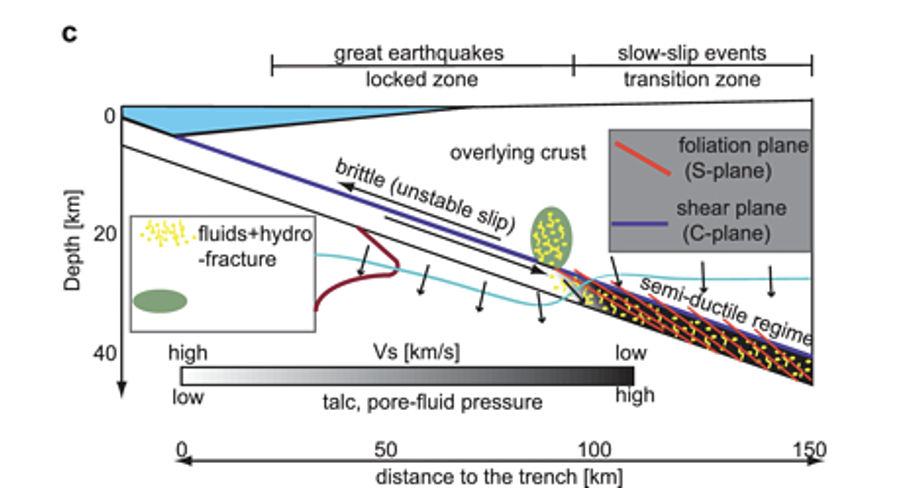
\includegraphics[width=6in]{SCanisotropy.png}
    \caption[墨西哥隱沒帶板塊介面附近剪切帶結構示意圖,摘自\citet{Song2012SC}]{墨西哥隱沒帶板塊介面附近剪切帶結構示意圖,摘自\citet{Song2012SC}。大地震主要發生在鎖定區(locked zone)和脆性(brittle)變形區域。慢速滑移事件(slow-slip event)主要發生在過渡帶(transition zone)和半韌性區域(seni-ductile regime),V$_S$非常低,且非均向性極強。這些低速帶流體導致板塊介面處於弱耦合狀態,並且主導該地區慢速滑移事件的生成。
    }
    \label{fig::SCanisotorpy2012}
\end{figure*}

%\begin{figure*}[ht!]
%    \centering
%    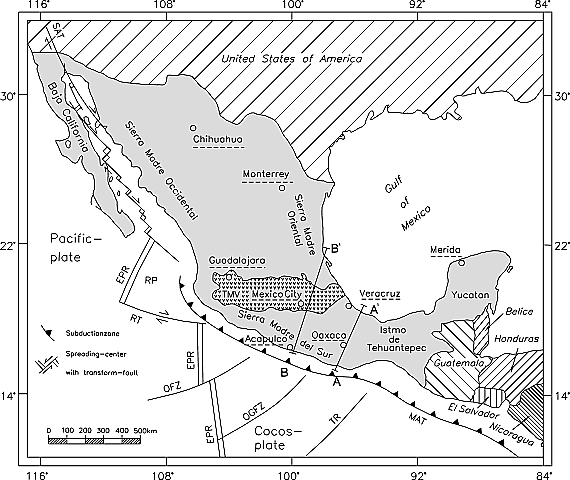
\includegraphics[width=3in]{MT_line.png}
%    \caption{\citealp{MT2006}中所使用的大地電磁剖面位置圖,本研究僅使用BB'剖面。
%    }
%    \label{fig::MT_site}
%\end{figure*}

\begin{figure*}[ht!]
    \centering
    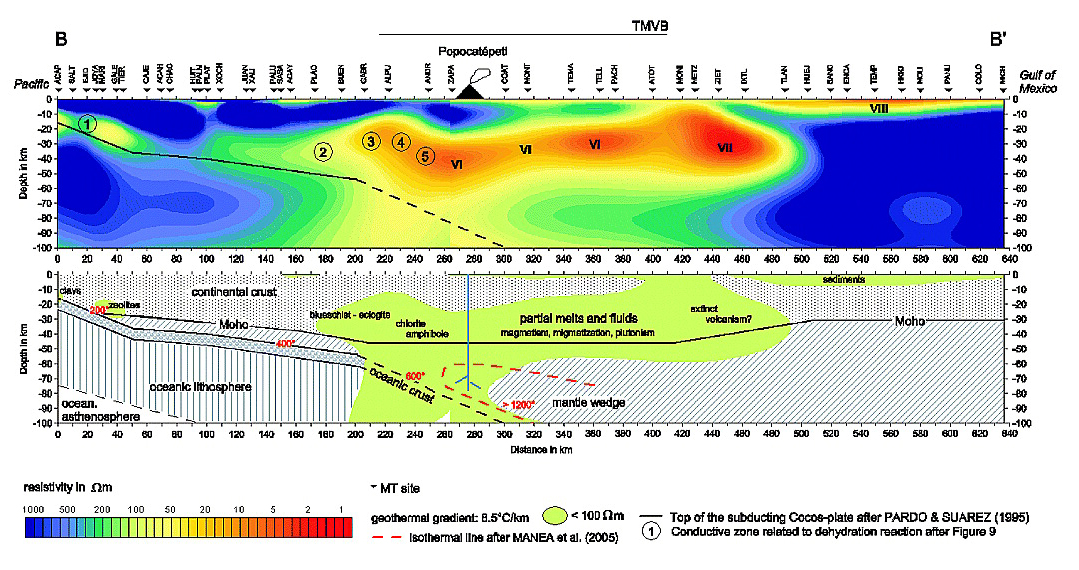
\includegraphics[width=6in]{MT_profile.png}
    \caption[墨西哥平坦隱沒區域的導電率異常剖面圖與解釋圖,摘自\citet{MT2006}]{墨西哥平坦隱沒區域的導電率異常剖面圖與解釋圖,摘自\citet{MT2006}。上圖為電阻率異常結果剖面,所繪之隱沒板塊位置參考自\citet{pardo1995}結果,最上方標示跨墨西哥火山帶的範圍。圖中每個數字圈皆代表隱沒帶上岩石發生脫水的位置,1為黏土礦物的脫水,2為藍片岩相變至綠簾石發生的脫水,3為綠簾石相變至榴輝岩的脫水,4為隱沒板塊上綠泥石的脫水,5為角閃石的脫水。下圖為電阻異常解釋圖,綠色區域為電阻異常低區(<100 $\Omega m$)。在平坦隱沒段結束處有多個岩石相變事件發生,隱沒板塊上出現大範圍導體。
    }
    \label{fig::MT_profile}
\end{figure*}

\citet{MT2006}利用大地電磁法獲得墨西哥平坦隱沒區域的導電率異常剖面(見圖\ref{fig::MT_profile}),發現在平坦隱沒結束前、隱沒板塊上方存在高導體區域,可能是隱沒板塊上物質因大量脫水產生。
圖\ref{fig::MT_profile}中編號2-5的弧前高導體區域與慢速滑移事件位置相吻合,表明該區域富含大量流體。
大量流體存在意味著脫水作用活躍,在隱沒板塊進入較高溫高壓環境下,釋放出的水分進入地函楔中,導致蛇紋岩化橄欖岩的生成。
對此,\citet{Manea2013}認為低速層可能不完全是地殼物質,而是過去因大量脫水而殘留下的地函蛇紋化橄欖岩成份,然而其內容物目前尚未完全了解。

\section{隱沒系統中的岩漿作用}\label{隱沒系統中的岩漿作用}
地球內部中,岩漿作用形成機制非常複雜,涉及部分熔融、冷卻過程結晶分異作用等。
若要使用簡單物理概念解釋部分熔融的形成,可分為三種,分別為減壓、增溫與脫水,又可分別對應中洋脊(mid ocean ridge)、熱點(hot spot)與火山島弧(volcanic arc)等三種構造。
地函岩石的乾固相線通常不會與地溫梯度曲線相交,然而當發生地區性減壓作用,會導致岩石在溫度不變的情況下快速降低壓力,此時容易通過岩石固相線,發生部分熔融事件,代表構造為中洋脊。
當一區域突然有額外熱源增溫,亦會導致岩石環境通過其固相線,發生部分熔融事件,代表構造為熱點火山。
聚合板塊邊界將大量地表物質帶入地球內部,物質為了在高溫高壓區維持穩定態,在隱沒過程中釋放流體,流體改變地函岩石的固相線,導致部分熔融發生,代表構造為聚合板塊邊界的火山島弧。

地函部分熔融在溫度大於攝氏850$^{\circ}$以上容易達到固相線,岩石發生部分熔融後產生岩漿庫。
攝氏850$^{\circ}$等溫線通常距海溝水平方向上100公里左右、離地表深度80-120公里之間產生(\citealp{peacock1990fluid}; \citealp{hyndman2003serpentinization}),並會因隱沒板塊傾角大小不同而稍微有水平距離上的改變。
由此可知火山島弧的發育與隱沒板塊、地函楔的溫度狀態有強烈相關性。

平坦隱沒帶具有極端的低傾角隱沒板塊,其溫度構造與一般的隱沒帶差異甚大,因此在平坦隱沒的演化過程中,岩漿與火山作用在時間軸上會有顯著的空間變化。
平坦隱沒的低角度隱沒板塊於地函淺部趨近於水平移動,故地函楔中攝氏850$^{\circ}$等溫線會隨時間逐漸往內陸移動,亦即部分熔融發生位置會漸往內陸移動,此時上覆板塊會出現寬闊的火山帶(volcanic belt),火山帶位置從距海溝100公里延伸至400公里以上(\citealp{Gutscher2000A}; \citealp{Manea2017})。
並且,隨著平坦隱沒持續發育,溫暖的地函楔逐漸被隱沒板塊閉合,隱沒板塊上方溫度漸漸降低降低,導致火山活動度逐漸減少甚至消失(\citealp{Gutscher2000Bcan})。
除此之外,平坦隱沒帶中的熱構造因著時間軸上的演化,因此其所產生的火成岩地球化學特徵在時間軸上同樣會有顯著變化。

安地斯(Andes)山脈長約7000公里,由納茲卡板塊隱沒進入南美板塊所形成。
儘管火山島弧遍及整段安地斯山脈中,現今平坦隱沒區域上方的火山活動止於全新世早期,見圖\ref{fig::flat_slab_vol}。
秘魯區域的地球化學研究資料稀少,因此,本研究中以智利區域為主要討論範圍。
岩漿期反應了在27-20 Ma有相對較陡峭的隱沒板塊,20-9 Ma發生擠壓變形,並且在8-4 Ma之間火山島弧往內陸遷移,暗示著隱沒板塊傾角正在逐漸變淺,平坦隱沒上方的岩漿作用在5 Ma左右停止(\citealp{kay2002magmatism})。
智利區域的岩漿成分隨時間變化有SiO$_2$與K$_2$O逐漸升高的現象,且其岩漿組成變化範圍極大(\citealp{kay1988tertiary}; \citealp{kay2002magmatism}; \citealp{goss2013andean})。

在智利平坦隱沒區域最北段的火成岩地球化學特徵被歸類為埃達克岩(adakite),約略出現於8-3 Ma之間,如圖\ref{fig::Chile_adakite_map}b中黃色圈處。
\citet{Gutscher2000Bcan}嘗試提出一地溫梯度極高的大陸岩石圈模型,導致隱沒板塊發生平坦隱沒後,板塊頂部溫度達到攝氏700-800$^{\circ}$,此時隱沒板塊上的部分熔融便可輕易發生。
儘管\citet{Gutscher2000Bcan}解釋認為智利的埃達克岩是隱沒板塊熔融所造成,並且是平坦隱沒中的一個重要過程。
然而\citet{kay2002magmatism}、\citet{goss2013andean}卻認為平坦隱沒帶中的上覆板塊溫度無法達到如此高溫,因而提出埃達克岩的來源應為大陸地殼熔融,而非海洋地殼熔融的概念模型。
他們的證據建立在智利埃達克岩的同位素特徵,該結果顯示其內容物由高壓大陸地殼岩石成分(石榴子石, garnet)所主導(\citealp{kay2002magmatism})。
目前對於智利區域埃達克岩的成因還有很大的討論空間,本研究將會在\ref{平坦隱沒中的埃達克岩}章節中進行更詳細的討論。

墨西哥境內的跨墨西哥火山帶(Trans Mexico Volcanic Belt)橫跨東西向墨西哥,約在25 Ma前後生成,該時期與可能的平坦隱沒初始發育期有關。
跨墨西哥火山帶在中新世早期至中期(Early to Late Miocene, 19-8 Ma)的侵入岩以安山岩為主,可見圖\ref{fig::Mexico_adakite_map}墨西哥的火成岩分佈地圖。該時期火山島弧寬度從西向東有顯著側向變化,東北邊的岩漿作用逐漸遠離海溝,火山帶隨時間拉寬,導致火山島弧分佈與海溝呈現非平行的狀態,並且岩漿活動逐漸減小甚至消失。
地球化學分析認為該段時期的火成岩有隱沒流體量隨時間逐漸減少的特徵,並且安山岩的矽質成分逐漸變高,演變成英安岩(dacite)。
這個趨勢在15 Ma左右被侵入的埃達克岩中斷(\citealp{mori2007effects}),這些埃達克岩樣本被認為是隱沒板塊熔融的產物(\citealp{gomez2003temporal}; \citealp{mori2007effects}),埃達克岩會在\ref{平坦隱沒中的埃達克岩}章節中有詳細的討論。
總結來說,這段時間諸多地球化學特徵暗示著平坦隱沒正在發育,包含火成岩成分從玄武岩質安山岩(basaltic andesitic)逐漸變成英安岩、岩漿特徵隨時間演進有越來越多地殼的貢獻、岩漿作用與海溝的距離隨時間增加以及許多埃達克岩特徵的樣本出現。
平坦隱沒的發育止於11 Ma,此時火山島弧前緣(volcanic front)距海溝約450公里(\citealp{Manea2011Thermal})。
自11 Ma起火山島弧前緣開始以每百萬年10公里的速度往海溝移動,同時,鐵鎂質岩漿的成分開始變多,可能是平坦隱沒開始回捲(rollback)過程中,地函楔橄欖岩的減壓熔融產物(\citealp{gomez2003temporal})。
如今的火山島弧前緣約略與海溝距離350公里,有穩定活躍的火山活動現象。

\begin{figure*}[htp]
    \centering
    \includegraphics[width=6in]{Chile_adakite_map.pdf}
    \caption[智利火山分佈,摘自\citet{goss2009extreme}]{智利火山分佈,摘自\citet{goss2009extreme}。
    (a)南美洲西海岸和安第斯山脈主要構造形態特徵示意圖,改編自\citet{lamb2003cenozoic}。虛線為國界。黑色箭頭表示\citet{demets1990current}的平均聚合速度。板塊等深度線為灰色粗線,海拔高度2000公尺以上區域以橘色表示。三角形標示出活火山位置,NVZ = 北部火山區,CVZ = 中部火山區,SVZ = 南部火山區。黃色陰影框表示北部平坦隱沒區與過度區(27.5°–28.5°S)。
    (b)顯示圖(a)中黃色陰影框地圖。黑色實線為現代中部火山島弧位置,黑色短虛線為中新世火山島弧弧前位置。中生代火山島弧寬度由黑細線標出範圍。中生代火山島弧的侏羅紀 La Negra 玄武岩和輝長岩的露頭以灰色陰影顯示,新近紀玄武質火山活動地點由白星表示。黑色箭頭顯示約 50 公里的晚中新世火山島弧向東遷移。埃達克質火山活動區域由黃色圈圈表示,包括約 8 Ma Dos Hermanos lava、7-6 Ma與6-3 Ma的Pircas Negras和 3-2 Ma 的 Rio Salado Pircas Negras。
    }
    \label{fig::Chile_adakite_map}
\end{figure*}

\begin{figure*}[ht!]
    \centering
    \includegraphics[width=6in]{Mexico_map_adakite.pdf}
    \caption[中新世早期至晚期跨墨西哥火山帶火成岩分佈,摘自\citet{ferrari2012dynamic}]{中新世早期至晚期跨墨西哥火山帶火成岩分佈,摘自\citet{ferrari2012dynamic}。其中,黃色圈起處的火山為具有埃達克岩組成的火山。圓點表示\ref{平坦隱沒中的埃達克岩}節中圖\ref{fig::Cocos_geochemisty}進行地球化學分析的樣本位置,星星表示進行定年分析的樣本位置。紅圈圈處的Chalcalzingo domes為20 Ma前後出現的流紋岩樣本,具有非常高矽質埃達克岩成份,被視為該區最早的火成岩樣本,並且其成份為幾乎無雜質的隱沒板塊熔融物質(\citealp{gomez2008origin})。
    }
    \label{fig::Mexico_adakite_map}
\end{figure*}